\chapter{MODEL ANALYSIS}
\label{chap:model_analysis}

In this chapter, the numerical implementation of the model is probed.
First, the finite difference solution at several vertical resolutions
is compared to the exact solution in the case of a uniform medium with no scattering.
Then, kelp is added to introduce inhomogeneity in the medium, and light scattering is enabled.
The maximum feasible resolution for a finite difference solution is used as the ``true'' solution
and compared to lower resolutions to judge their performance.
Next, the low-scattering asymptotic approximation is compared to the finite difference solution
for the four sets of optical properties given in Table \ref{tab:petzold}.
Finally, several model parameters are varied from a base case to determine the model's sensitivity to each of them. 

\section{Homogeneous medium}
In this section, a homogeneous medium with $a_w=0.5$ and $b=0$ is used.
In the case of no scattering, the zeroth order asymptotic approximation
is in fact the true solution to the radiative transfer equation.
Several vertical grid spacings are used for a finite difference solution,
and resulting irradiance values are plotted at each depth layer.
Absolute and relative differences from the exact solution are shown.
Average errors are then plotted as a function of grid resolution.
For $n_z=24$, an average relative error of about 5\% is achieved.

\begin{figure}[H]
  \centering
  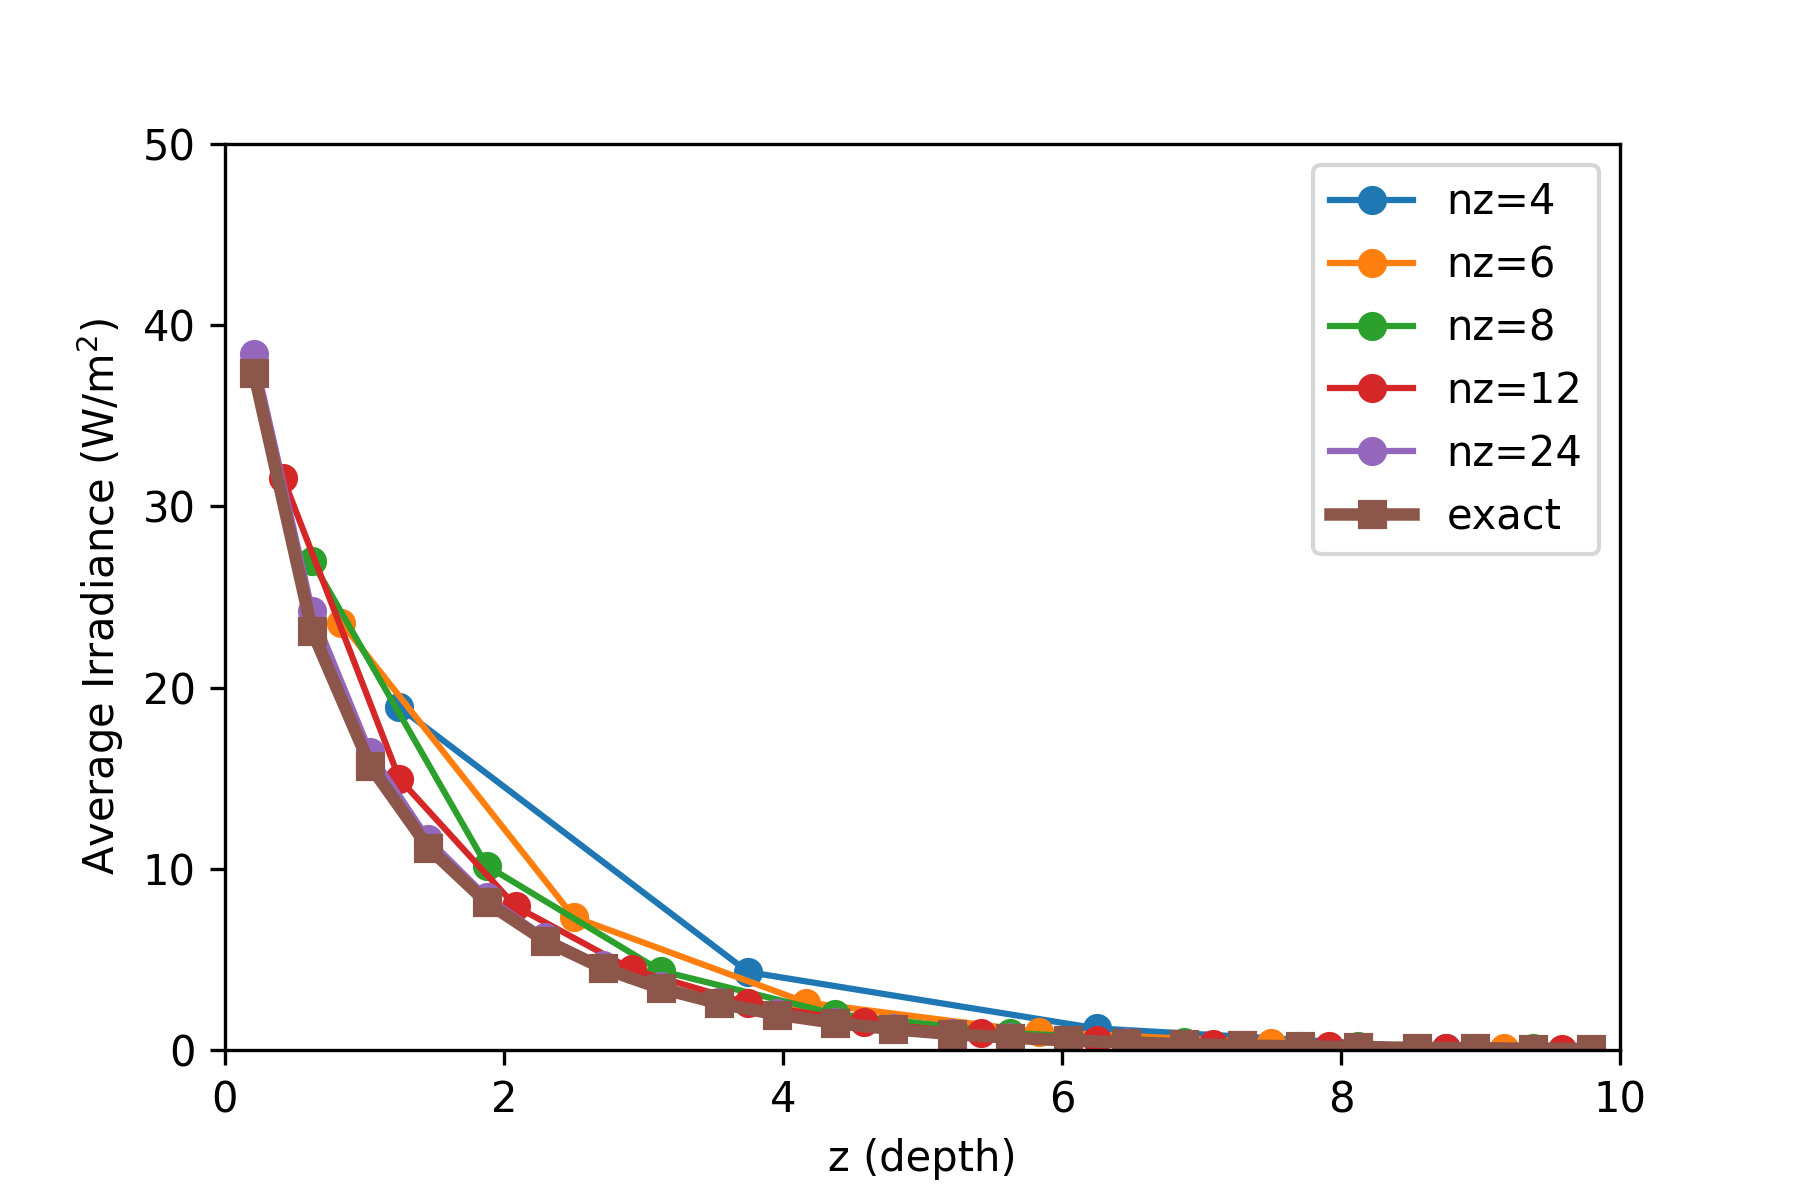
\includegraphics[width=4in]{exact_vs_fd_irrad}
  \caption{Exact v.s. finite difference irradiance, linear scale}
\end{figure}

\begin{figure}[H]
  \centering
  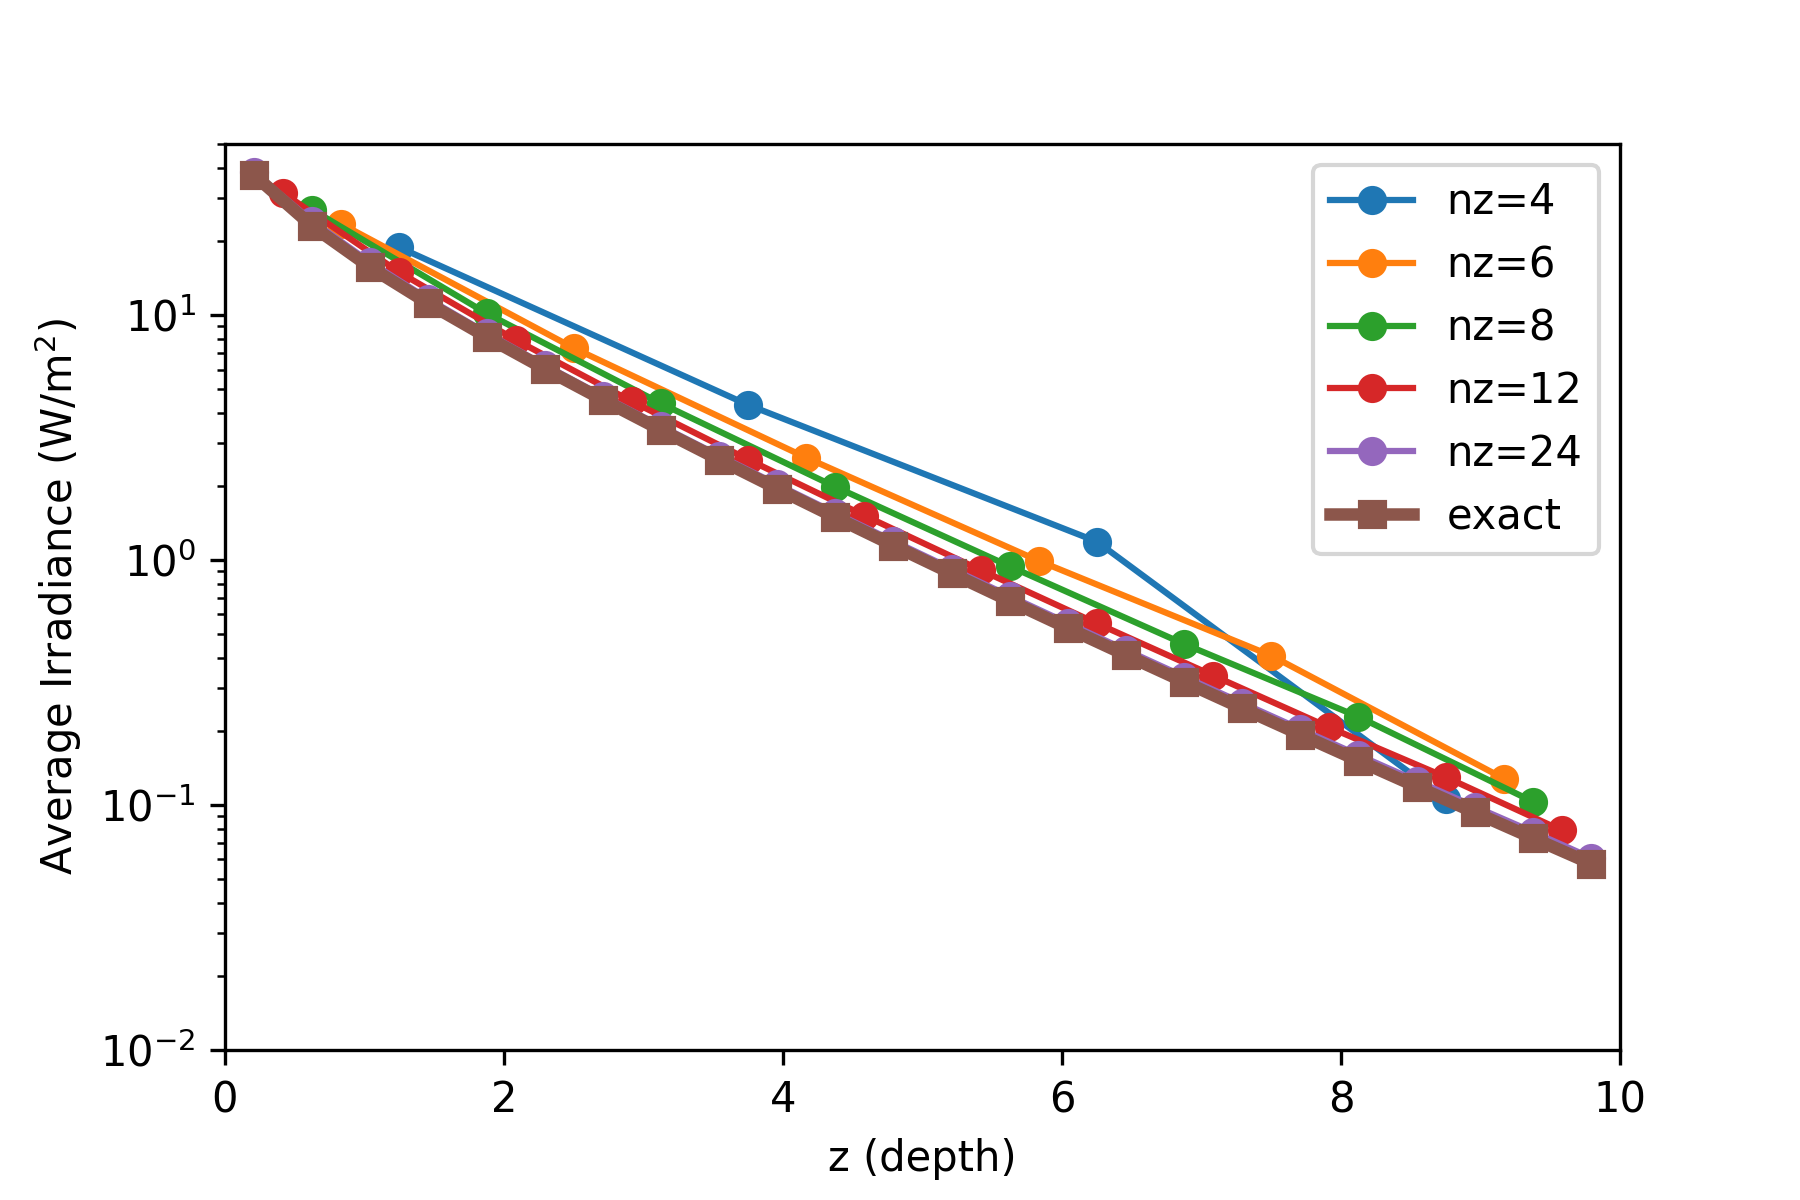
\includegraphics[width=4in]{exact_vs_fd_log_irrad}
  \caption{Exact v.s. finite difference irradiance, log scale}
\end{figure}

\begin{figure}[H]
  \centering
  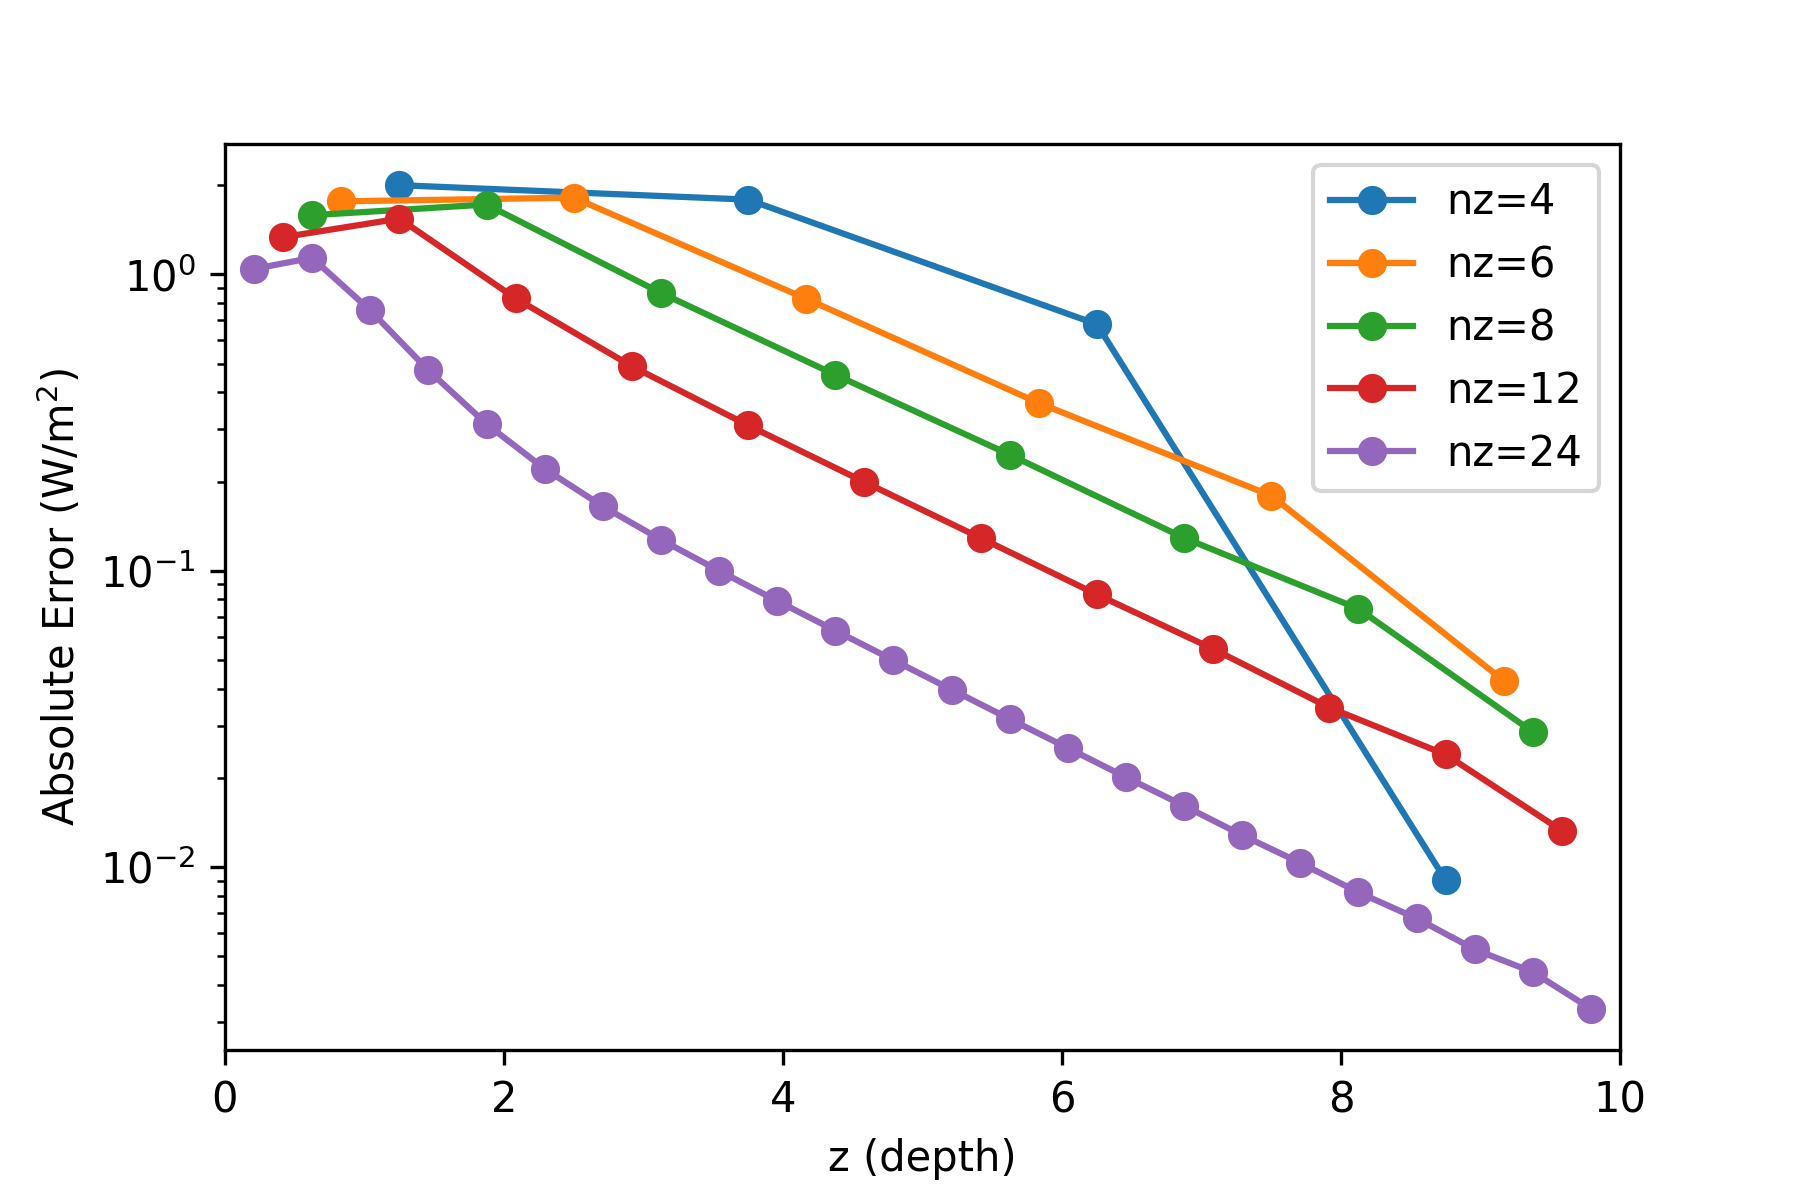
\includegraphics[width=4in]{exact_vs_fd_abs_err}
  \caption{Exact v.s. finite difference irradiance, absolute error}
\end{figure}

\begin{figure}[H]
  \centering
  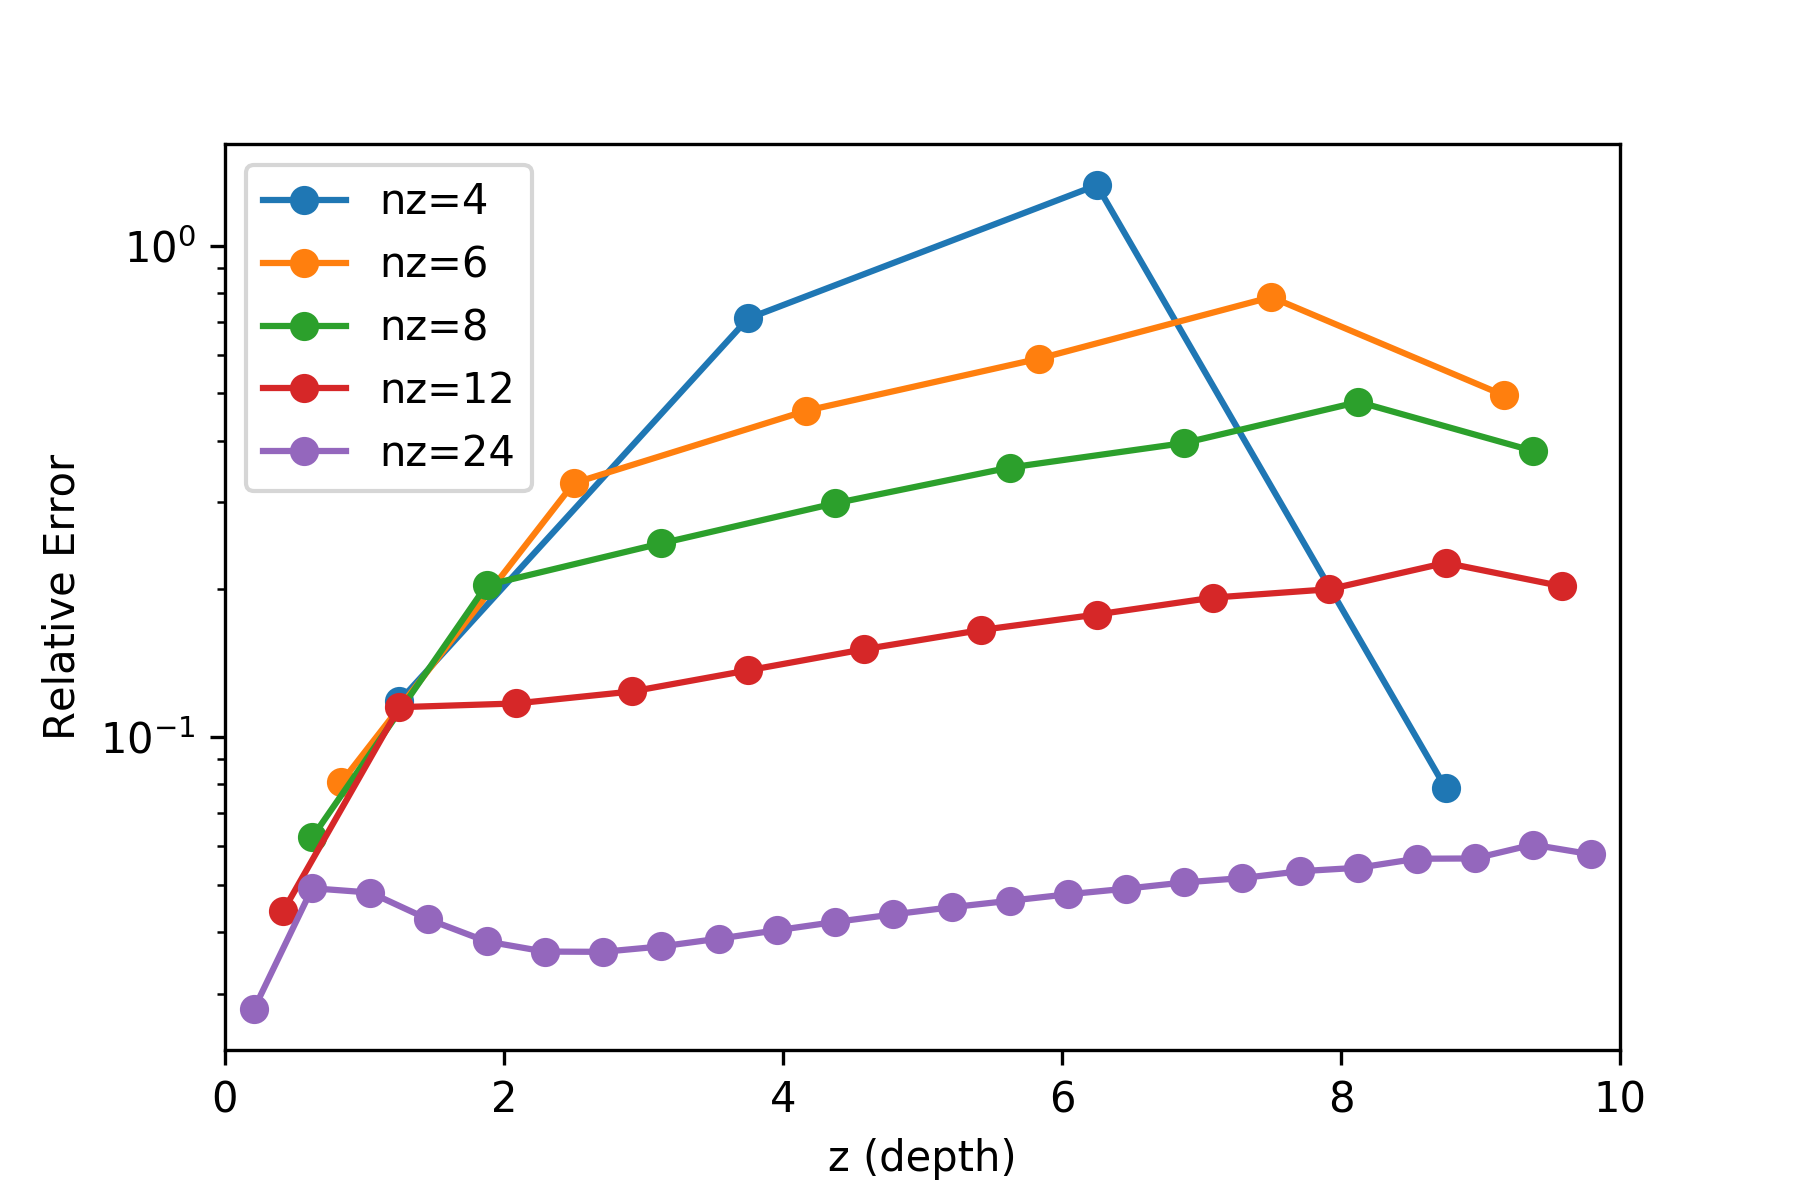
\includegraphics[width=4in]{exact_vs_fd_rel_err}
  \caption{Exact v.s. finite difference irradiance, relative error}
\end{figure}

\begin{figure}[H]
  \centering
  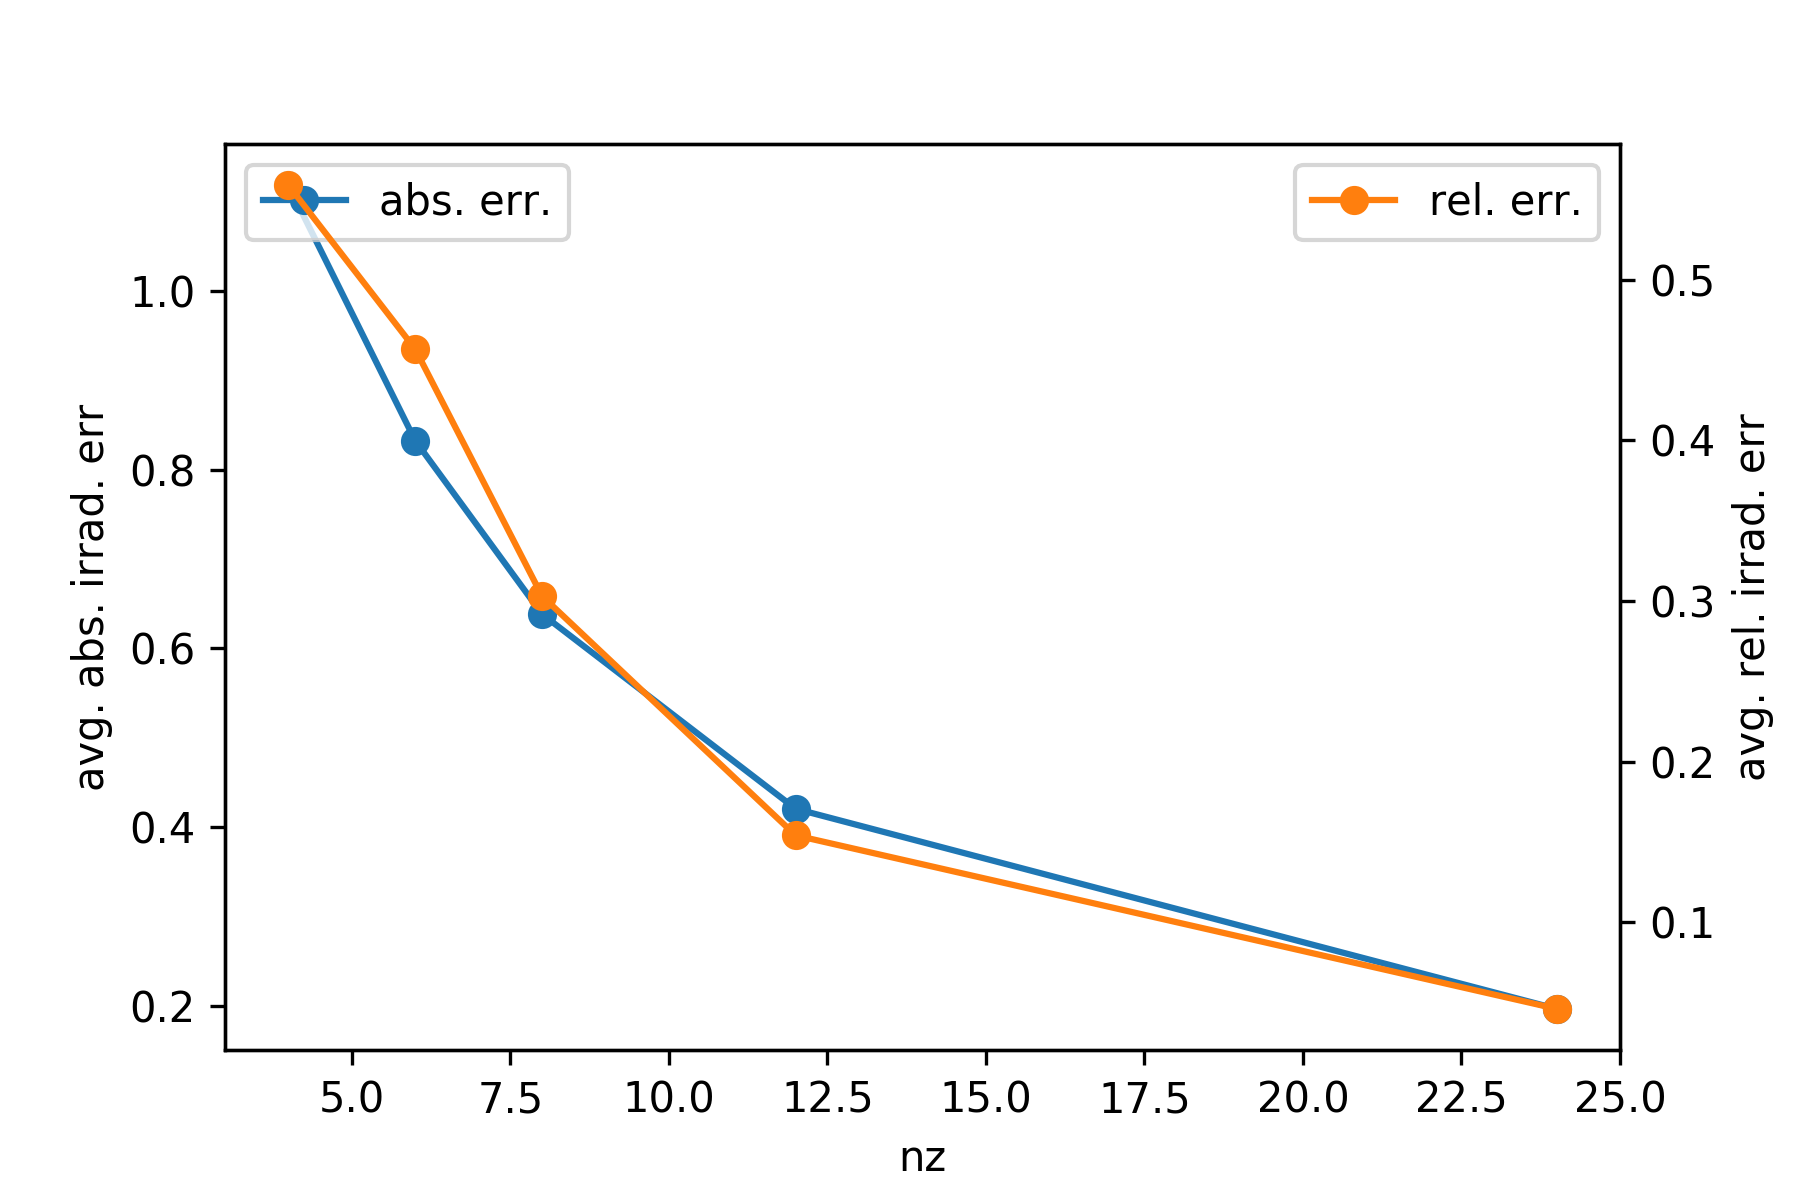
\includegraphics[width=4in]{exact_vs_fd_compare}
  \caption{Exact v.s. finite difference irradiance, relative error v.s. grid resolution}
\end{figure}

\section{Grid Study}
A five dimensional $(x,y,x,\theta,\phi)$ resolution space is nontrivial to characterize.
For the sake of reducing dimensionality, we define generic spatial and angular resolutions
$n_s$ and $n_a$ such that $n_s=n_x=n_y$ and $n_a=n_\theta=n_\phi$.
Remaining is a three-dimensional resolution space, $(n_s,n_z,n_a)$.
Rather than perform calculations at every possible combination of resolutions in the space,
we choose a maximum resolution of $20 \times 20 \times 20$,
and hold two of the three resolutions at the maximum value while varying the third.
For example, Figure \ref{fig:gs_ns} compares $4 \times 20 \times 20$, $6 \times 20 \times 20$, $8 \times 20 \times 20$, etc.
The quantity that we compare is \textit{perceived irradiance}, which is different than the simple mean irradiance in each depth layer.
Rather, the average is weighted by the normalized spatial kelp distribution to determine the average irradiance experienced by the kelp population.
For more detail, see Section \ref{sec:perceived_irrad}

Note the different natures of convergence in each dimension.
In varying $n_s$, we see that the accuracy is very low for small $n_s$ values.
This is because in these cases, the horizontal grid cells are too large to capture any detail
about the kelp fronds near the bottom where they are very small.
The kelp is effectively not present in these layers, and therefore the perceived irradiance is zero.
After increasing the resolution past this minimum threshold, however, little improvement results
from increasing $n_s$ further, as seen in Figure \ref{fig:gs_ns}.
On the other hand, Figure \ref{fig:gs_nz} shows that increasing the vertical resolution
consistently improves the accuracy of the solution.
Figure \ref{fig:gs_na} shows that $n_a$ is somewhere between the two,
demonstrating clear improvement with increasing resolution, though the improvement is not uniform over depth.
Figure \ref{fig:gs_compare} shows the trend of increasing accuracy with increasing resolution in each dimension.

\begin{figure}[h]
  \centering
  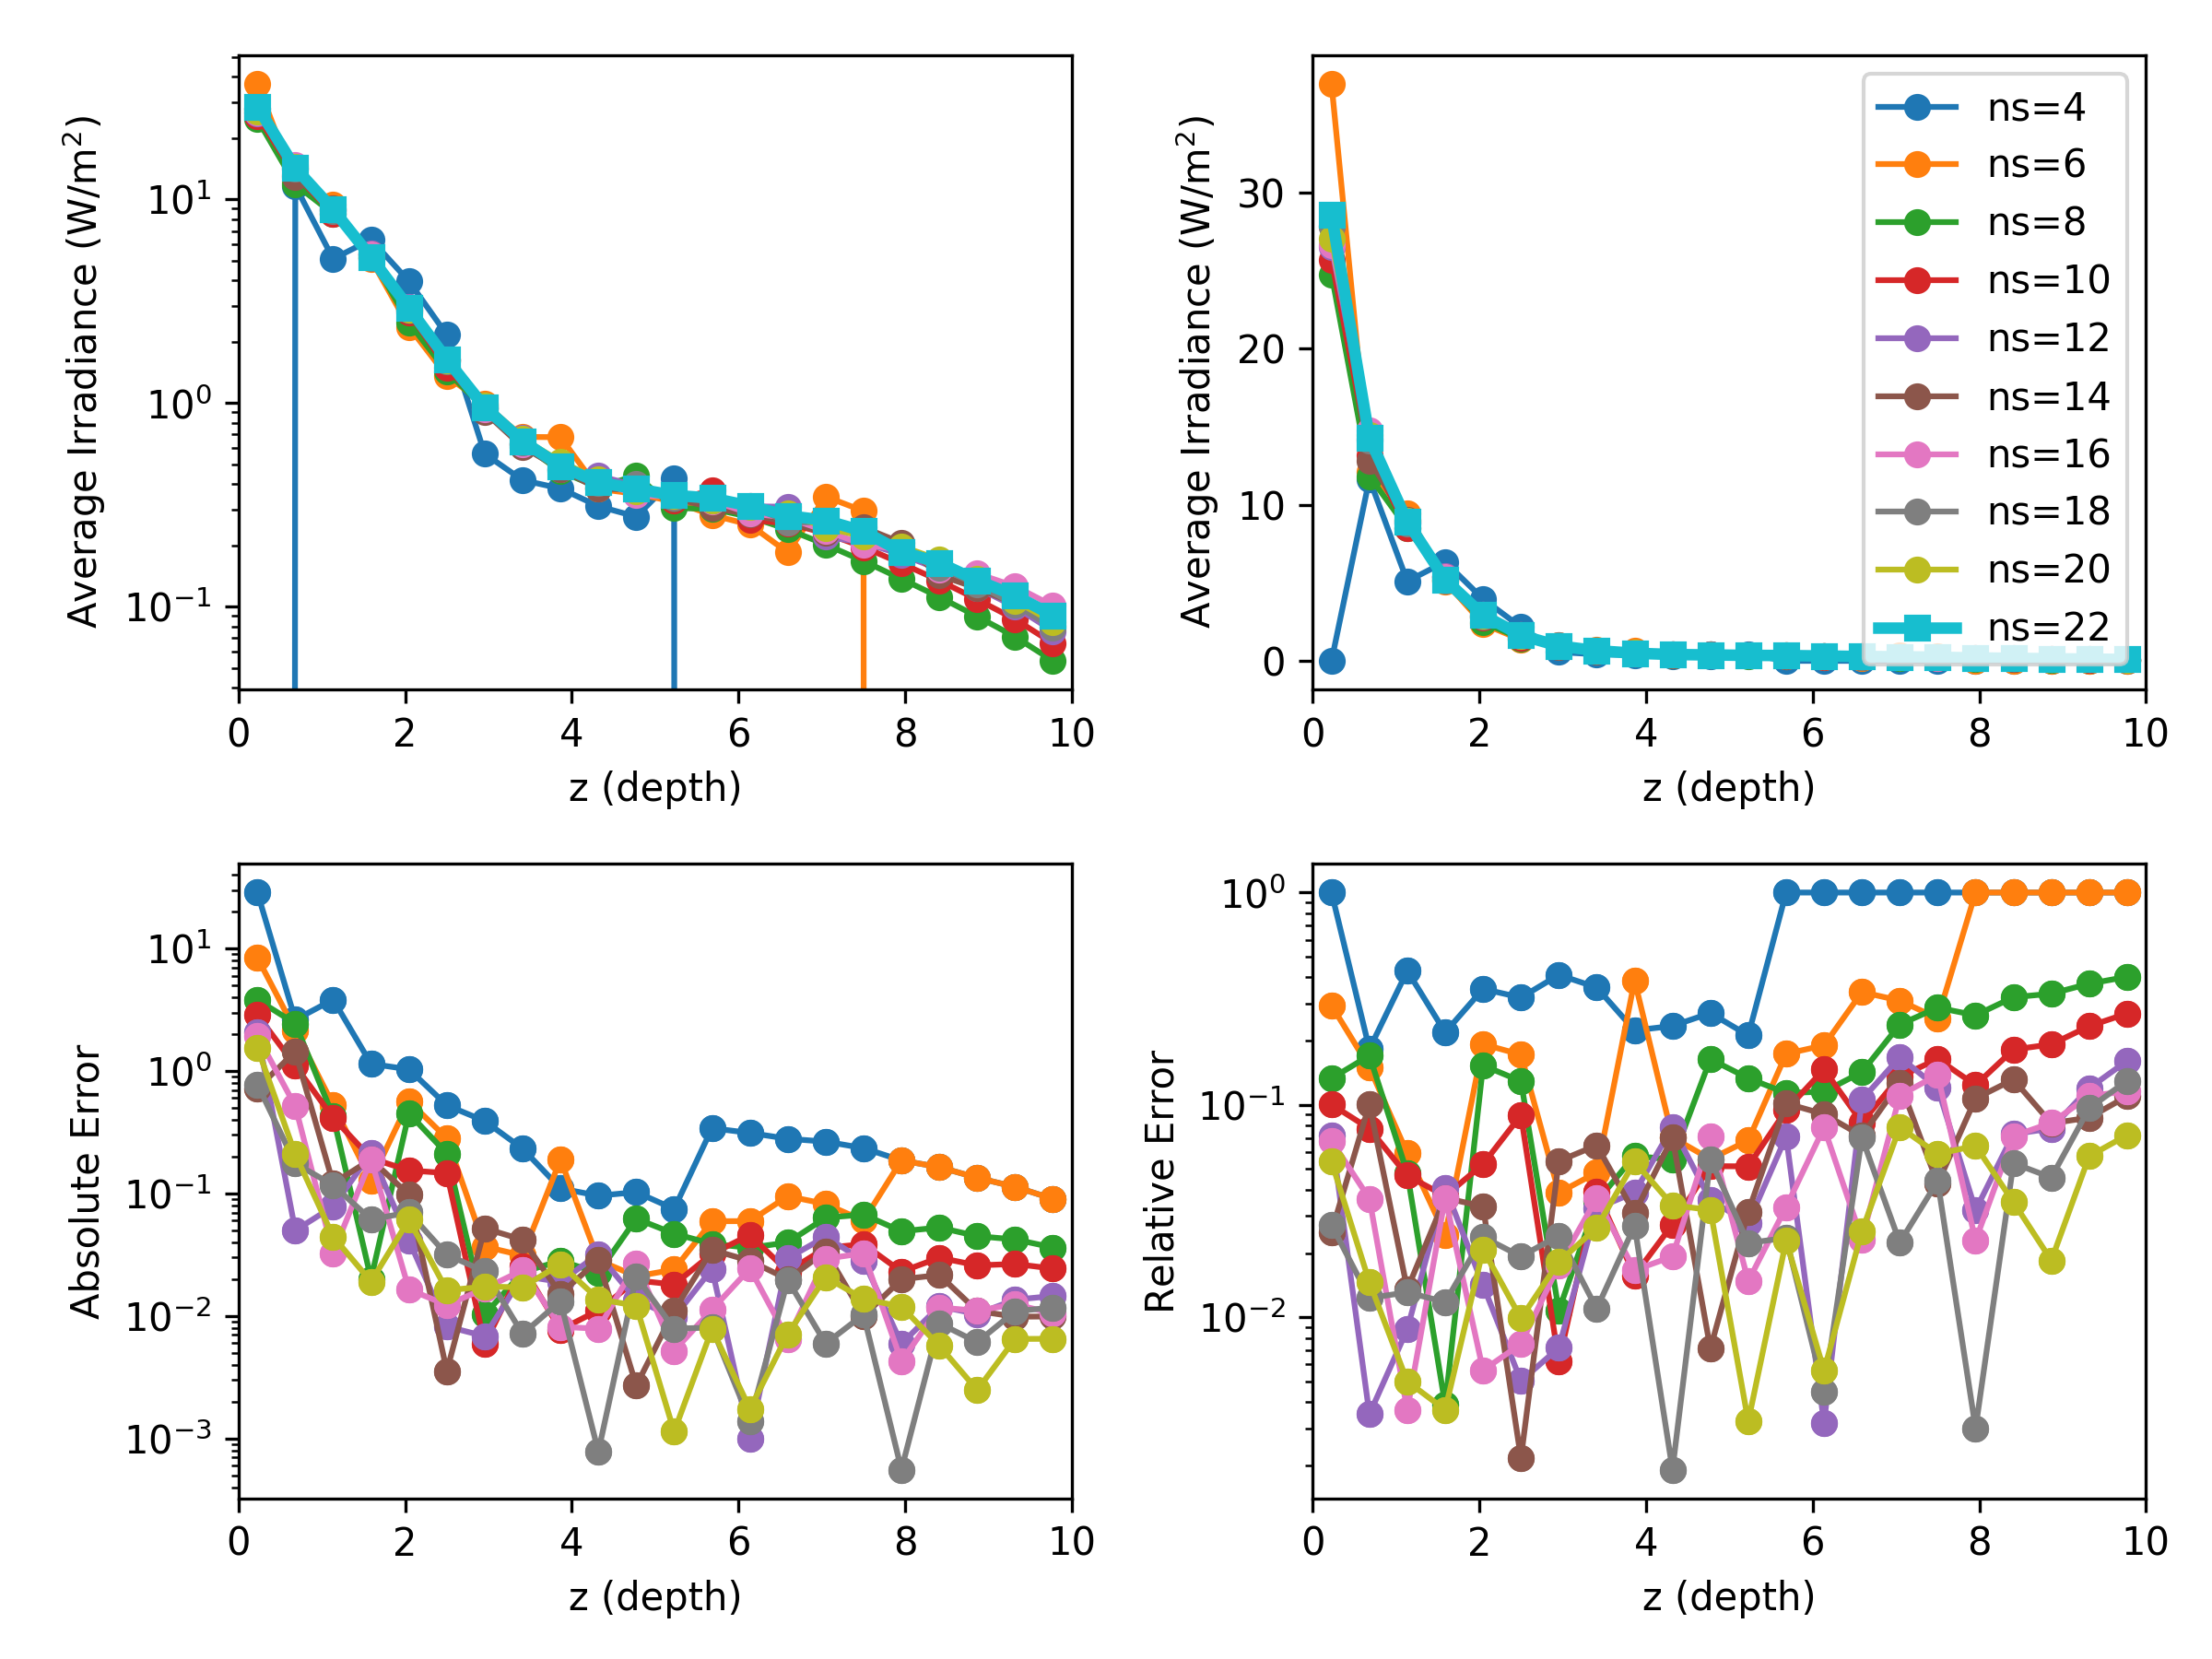
\includegraphics[width=\textwidth]{gs_ns}
  \caption{Grid study, $n_s$}
  \label{fig:gs_ns}
\end{figure}

\begin{figure}[h]
  \centering
  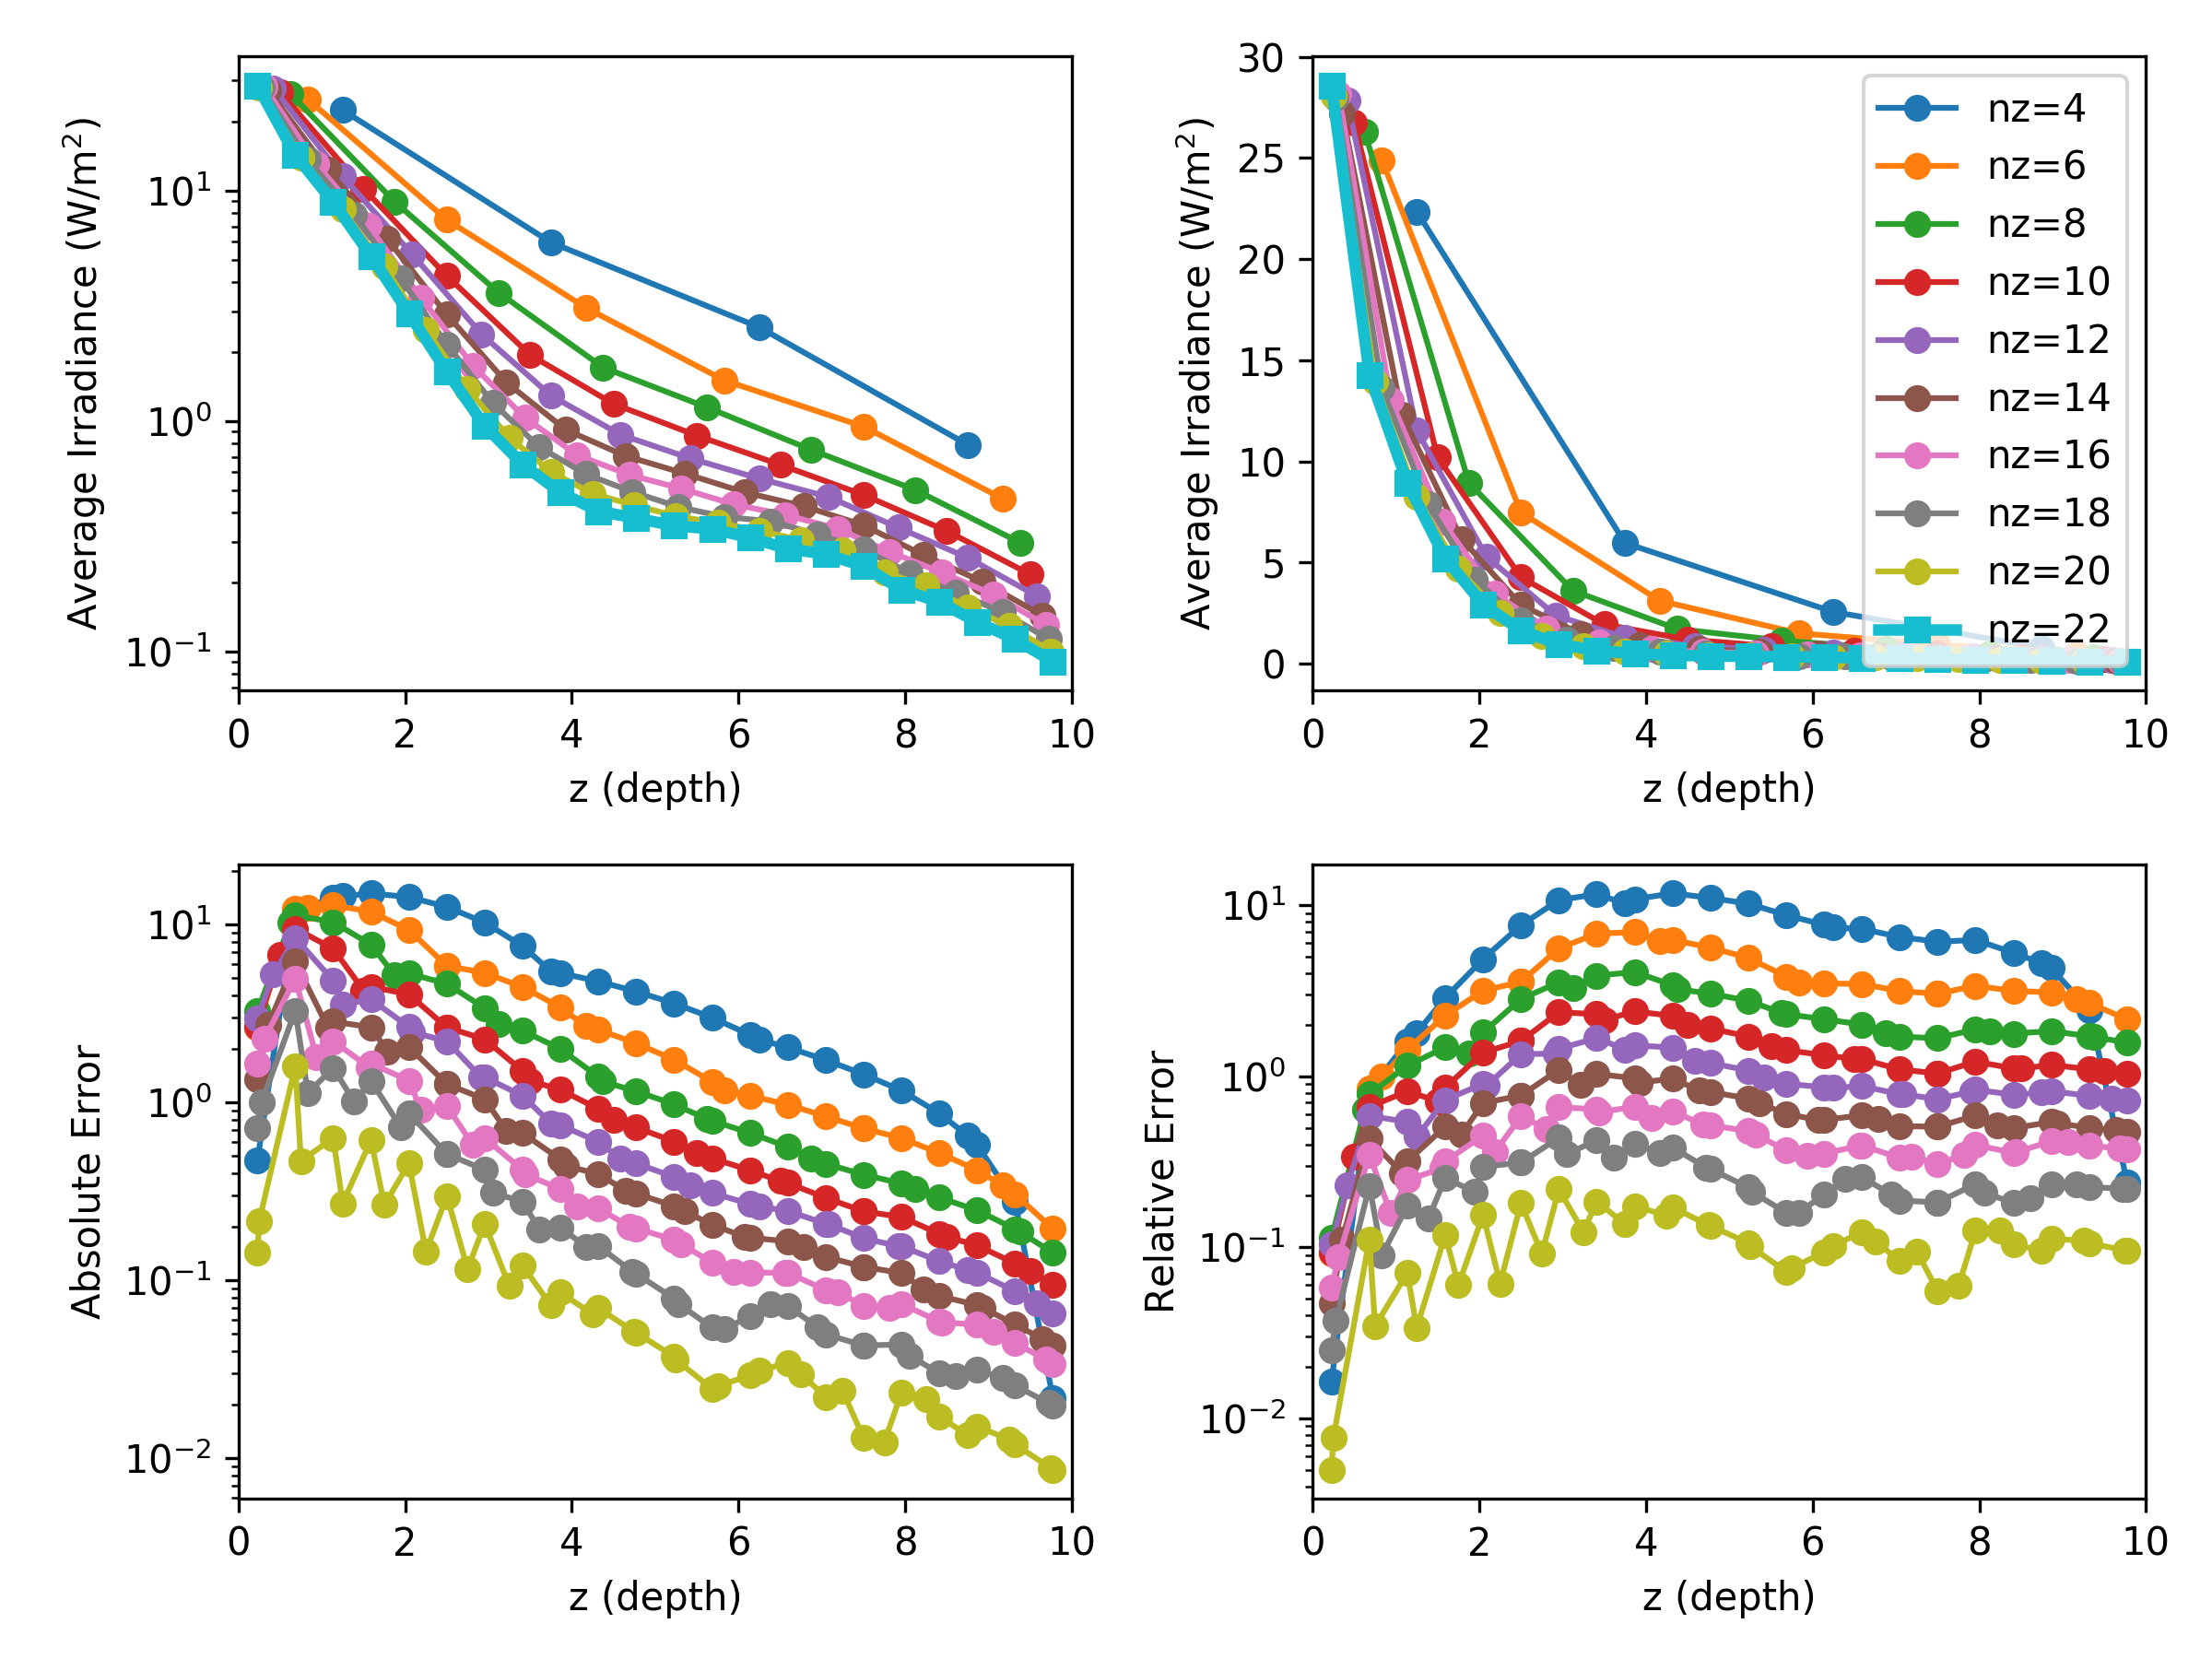
\includegraphics[width=\textwidth]{gs_nz}
  \caption{Grid study, $n_z$}
  \label{fig:gs_nz}
\end{figure}

\begin{figure}[h]
  \centering
  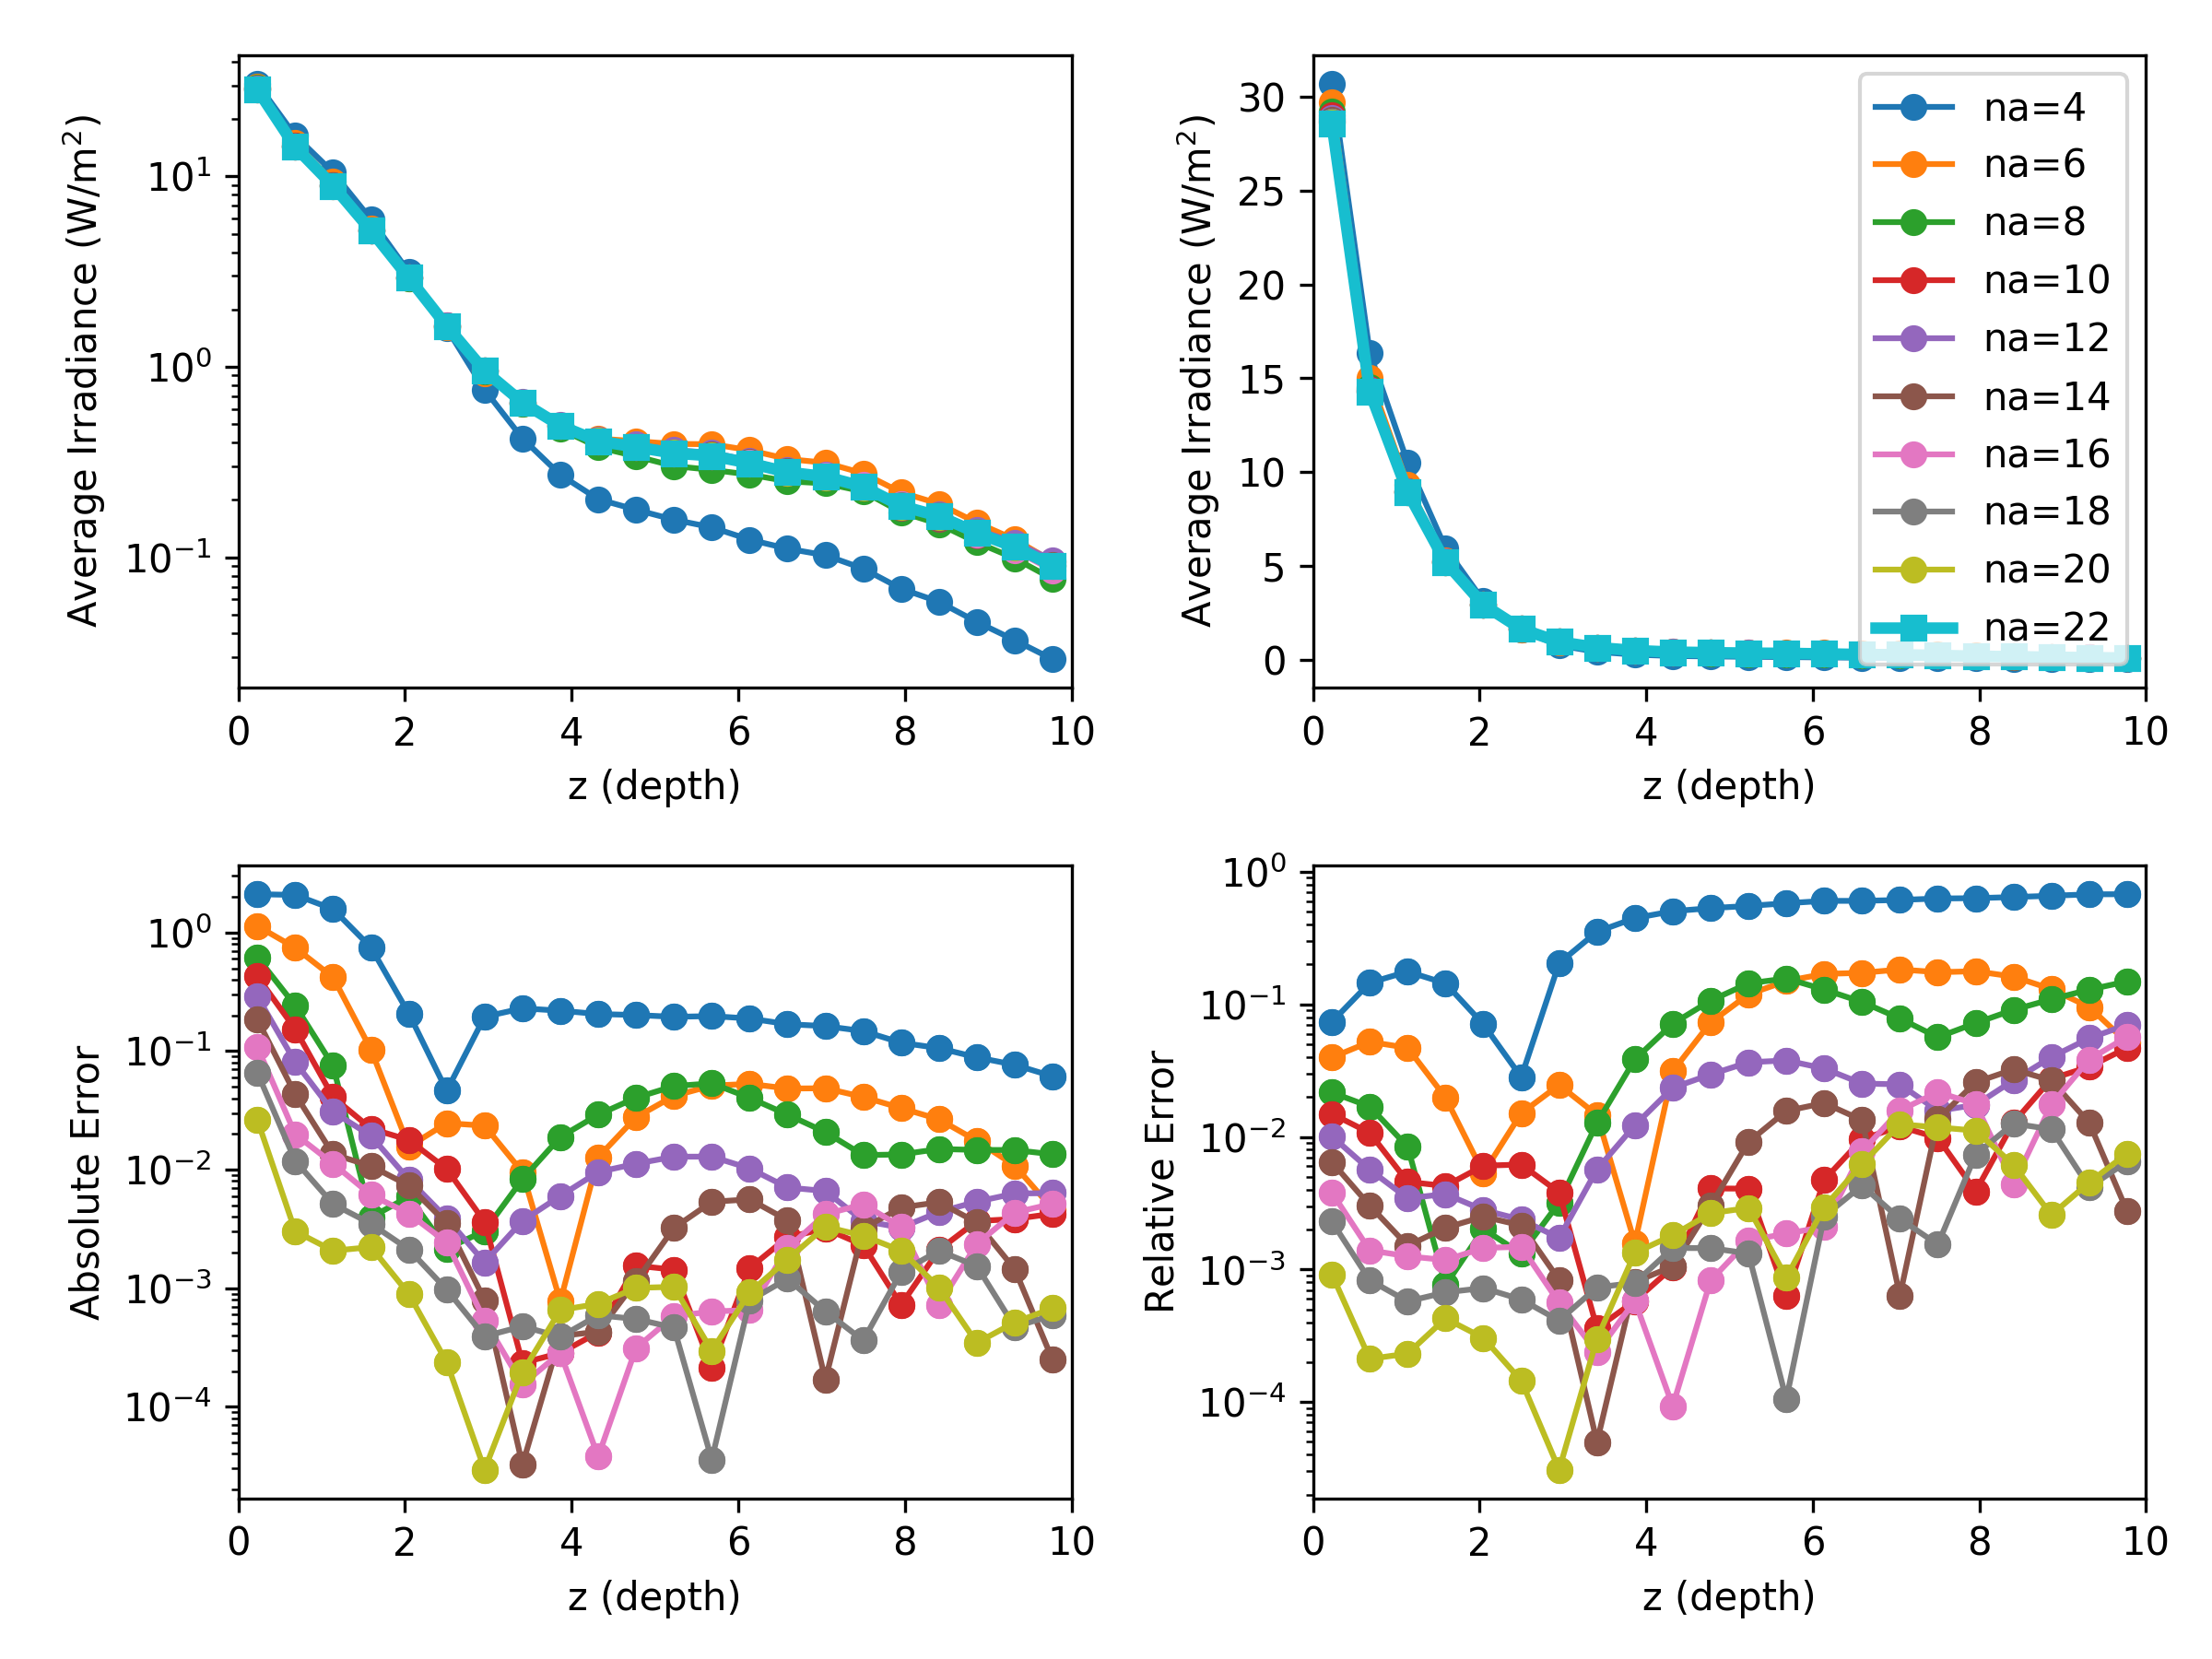
\includegraphics[width=\textwidth]{gs_na}
  \caption{Grid study, $n_a$}
  \label{fig:gs_na}
\end{figure}

\begin{figure}[h]
  \centering
  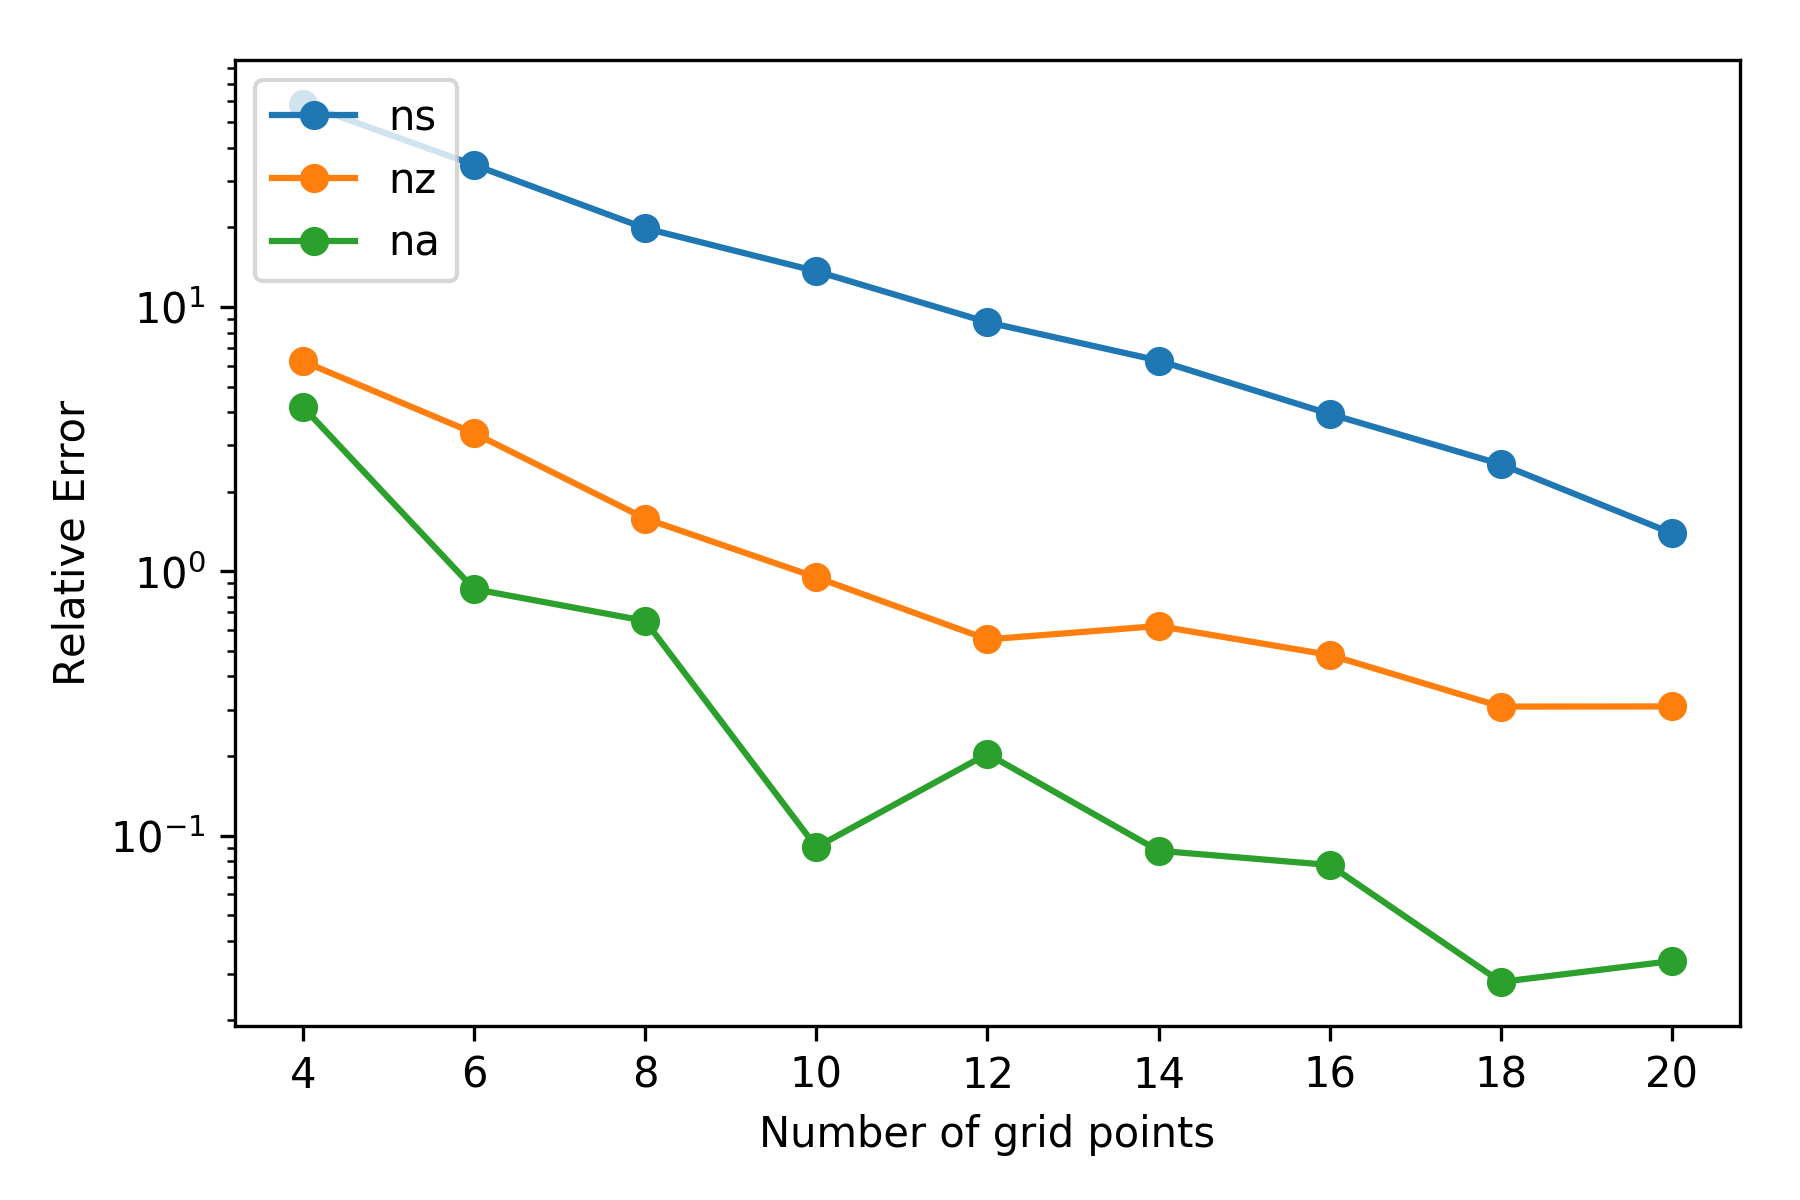
\includegraphics[width=4in]{gs_compare}
  \caption{Grid study, summary}
  \label{fig:gs_compare}
\end{figure}


\begin{figure}[h]
  \centering
  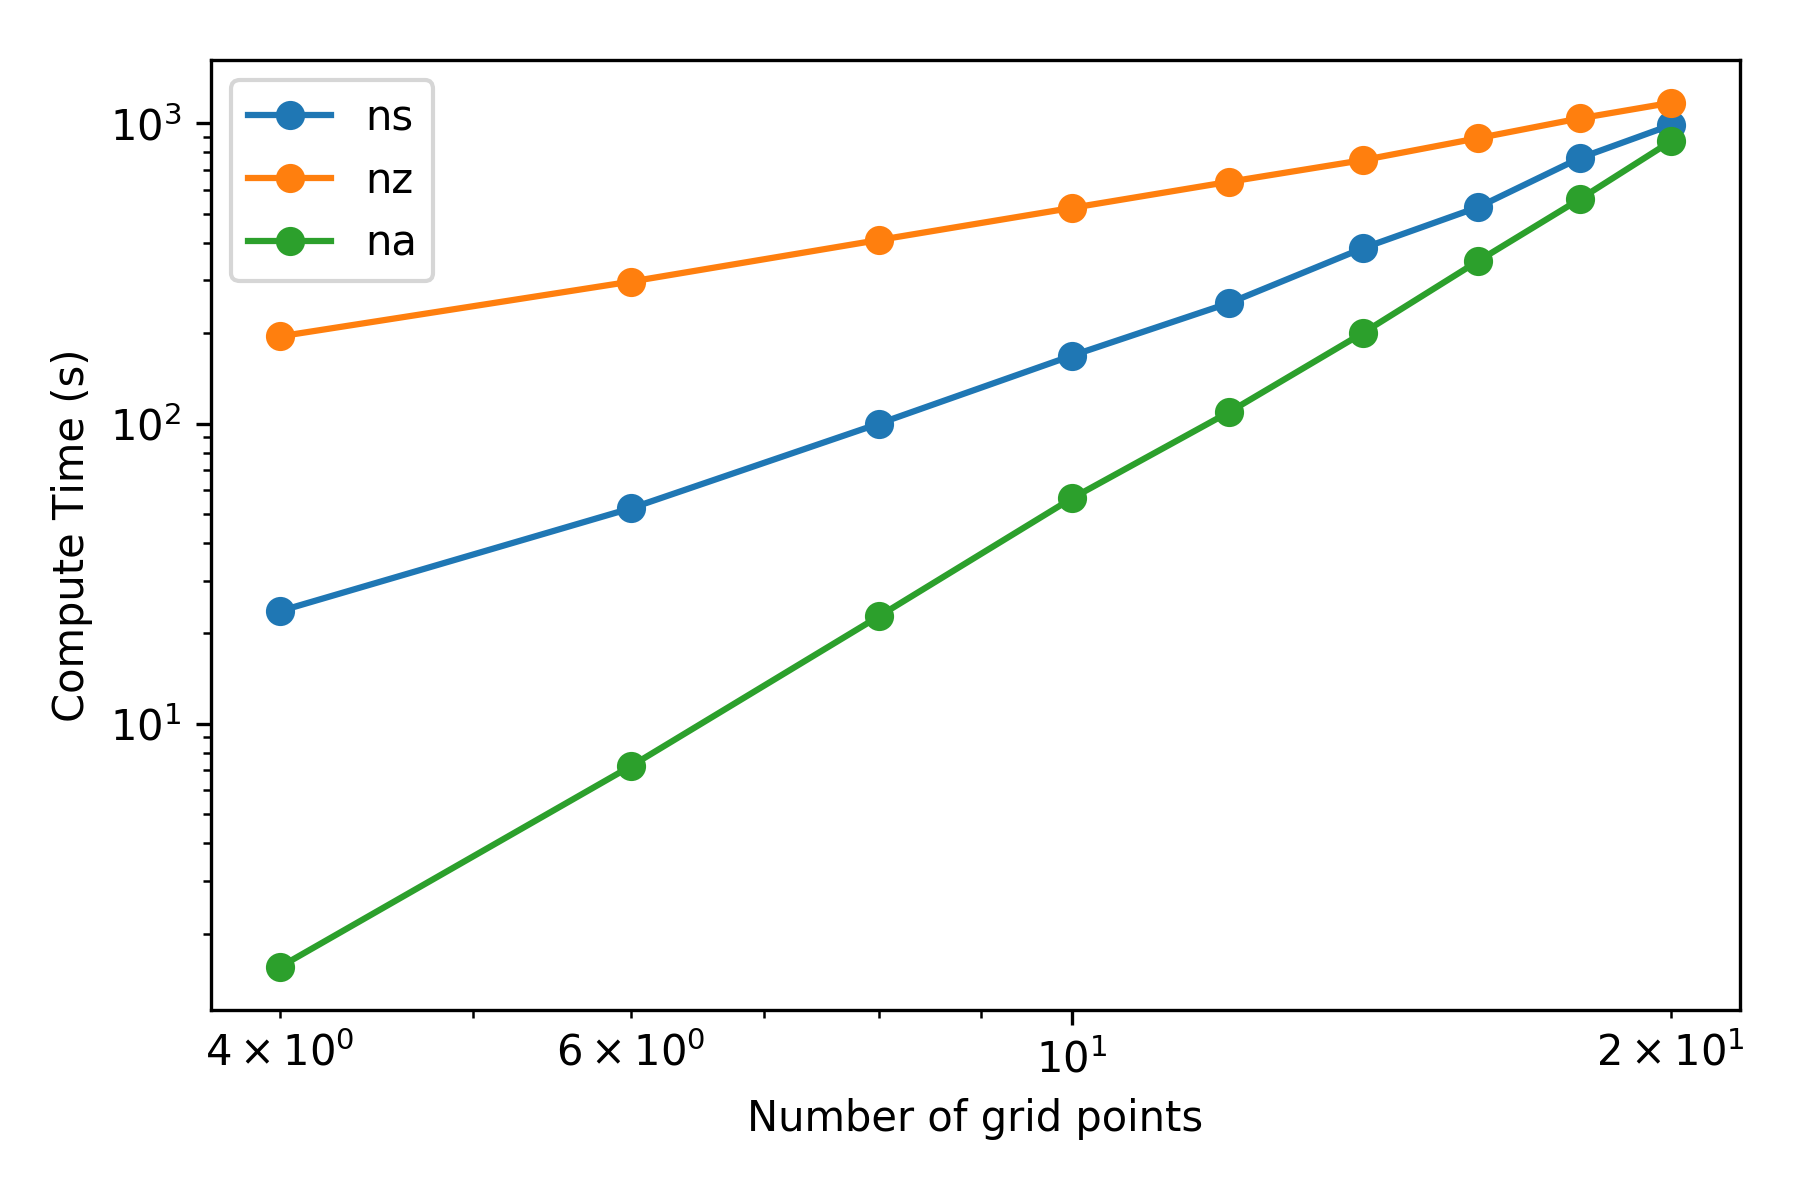
\includegraphics[width=4in]{gs_time}
  \caption{Grid study, time}
  \label{fig:gs_compare}
\end{figure}


\section{Asymptotic Convergence}
\label{sec:asym_conv}

In this section, the four water cases from Table \ref{tab:petzold} are considered.
In each case, the full finite difference solution is calculated on an $18 \times 18 \times 18$ grid,
and asymptotic approximations are given, varying the number of terms used in the asymptotic series.
Perceived irradiances are shown, as well as errors from the finite difference solution.

In the first two cases, when the scattering coefficient is the same order or smaller as the absorption coefficient,
the asymptotic approximation converges to the finite difference solution.
However, in the very turbid water of the San Diego Harbor, the scattering coefficient is an order of magnitude higher
than the absorption coefficient, causing the asymptotic solution to quickly diverge.
In figure \ref{fig:asym_conv_compare}, average relative errors for the two converging cases are shown.
In both cases, the accuracy improves with more scattering events until it plateaus.
In the first case, 4 scattering events is sufficient, whereas in the second, the accuracy improves until 12 scattering events.

\begin{figure}[H]
  \centering
  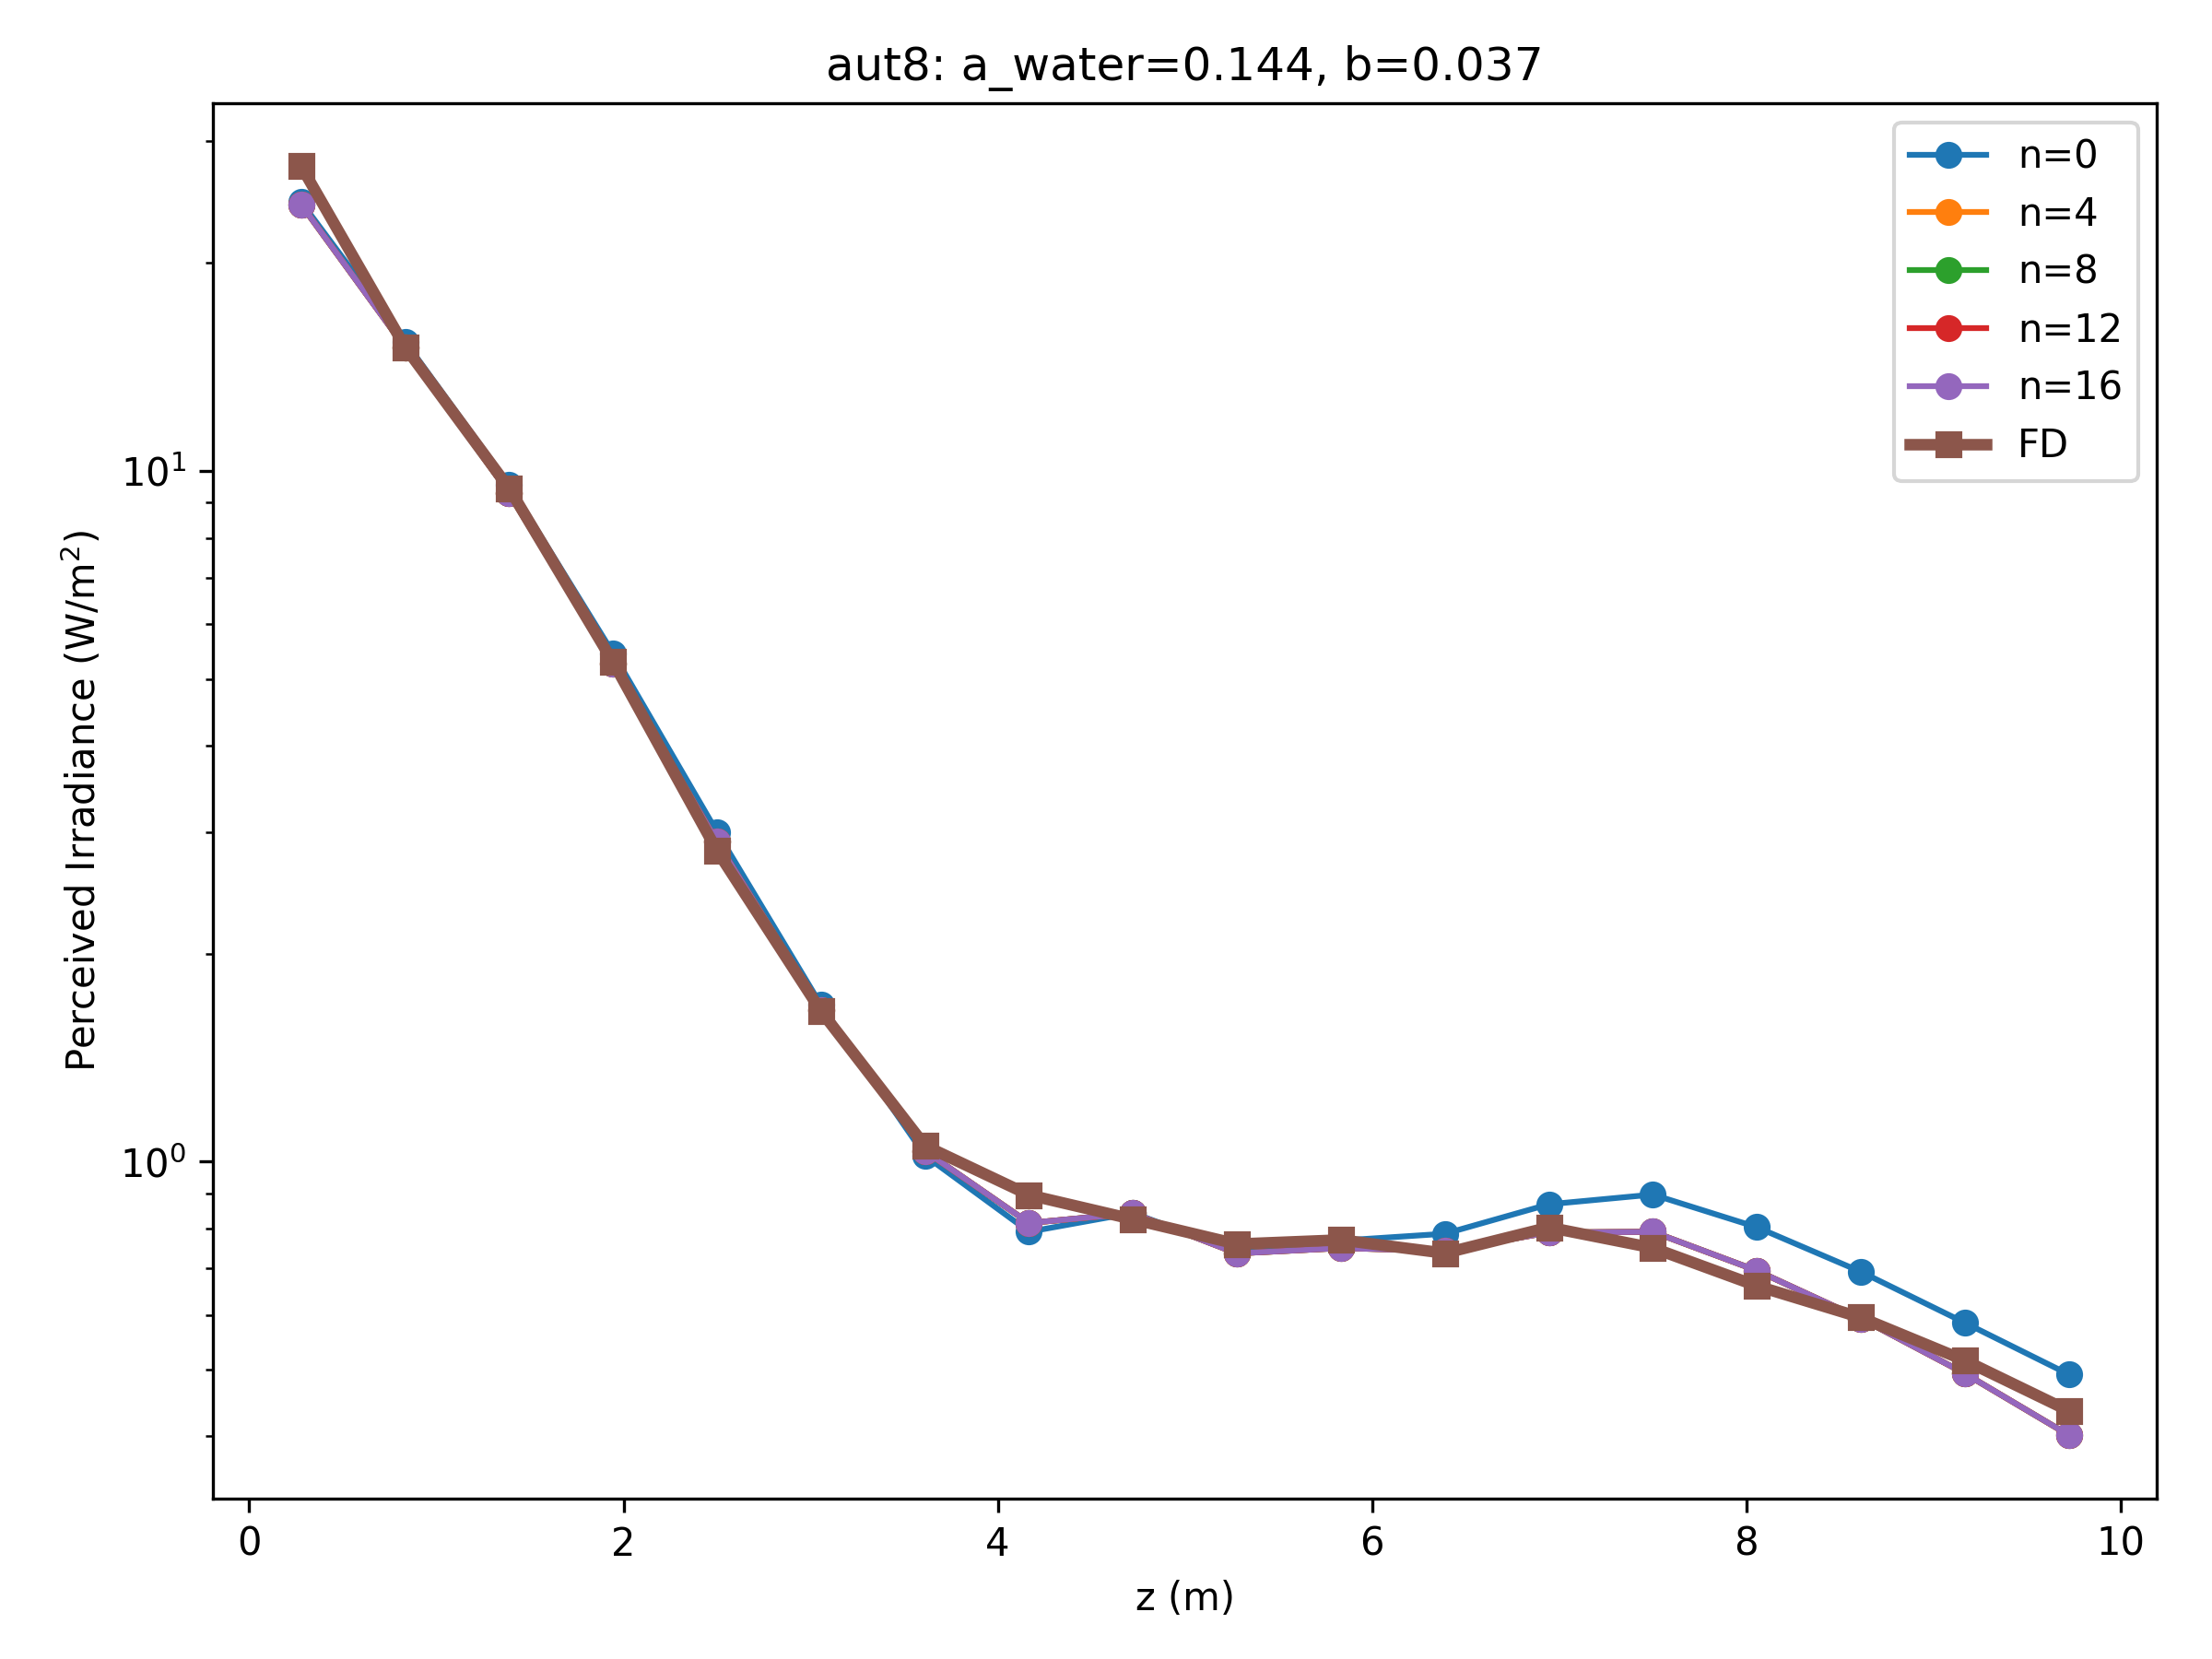
\includegraphics[width=4in]{asym_conv_irrad_aut8}
  \caption{Successive asymptotic approximations, irradiance: AUT8}
\end{figure}

\begin{figure}[H]
  \centering
  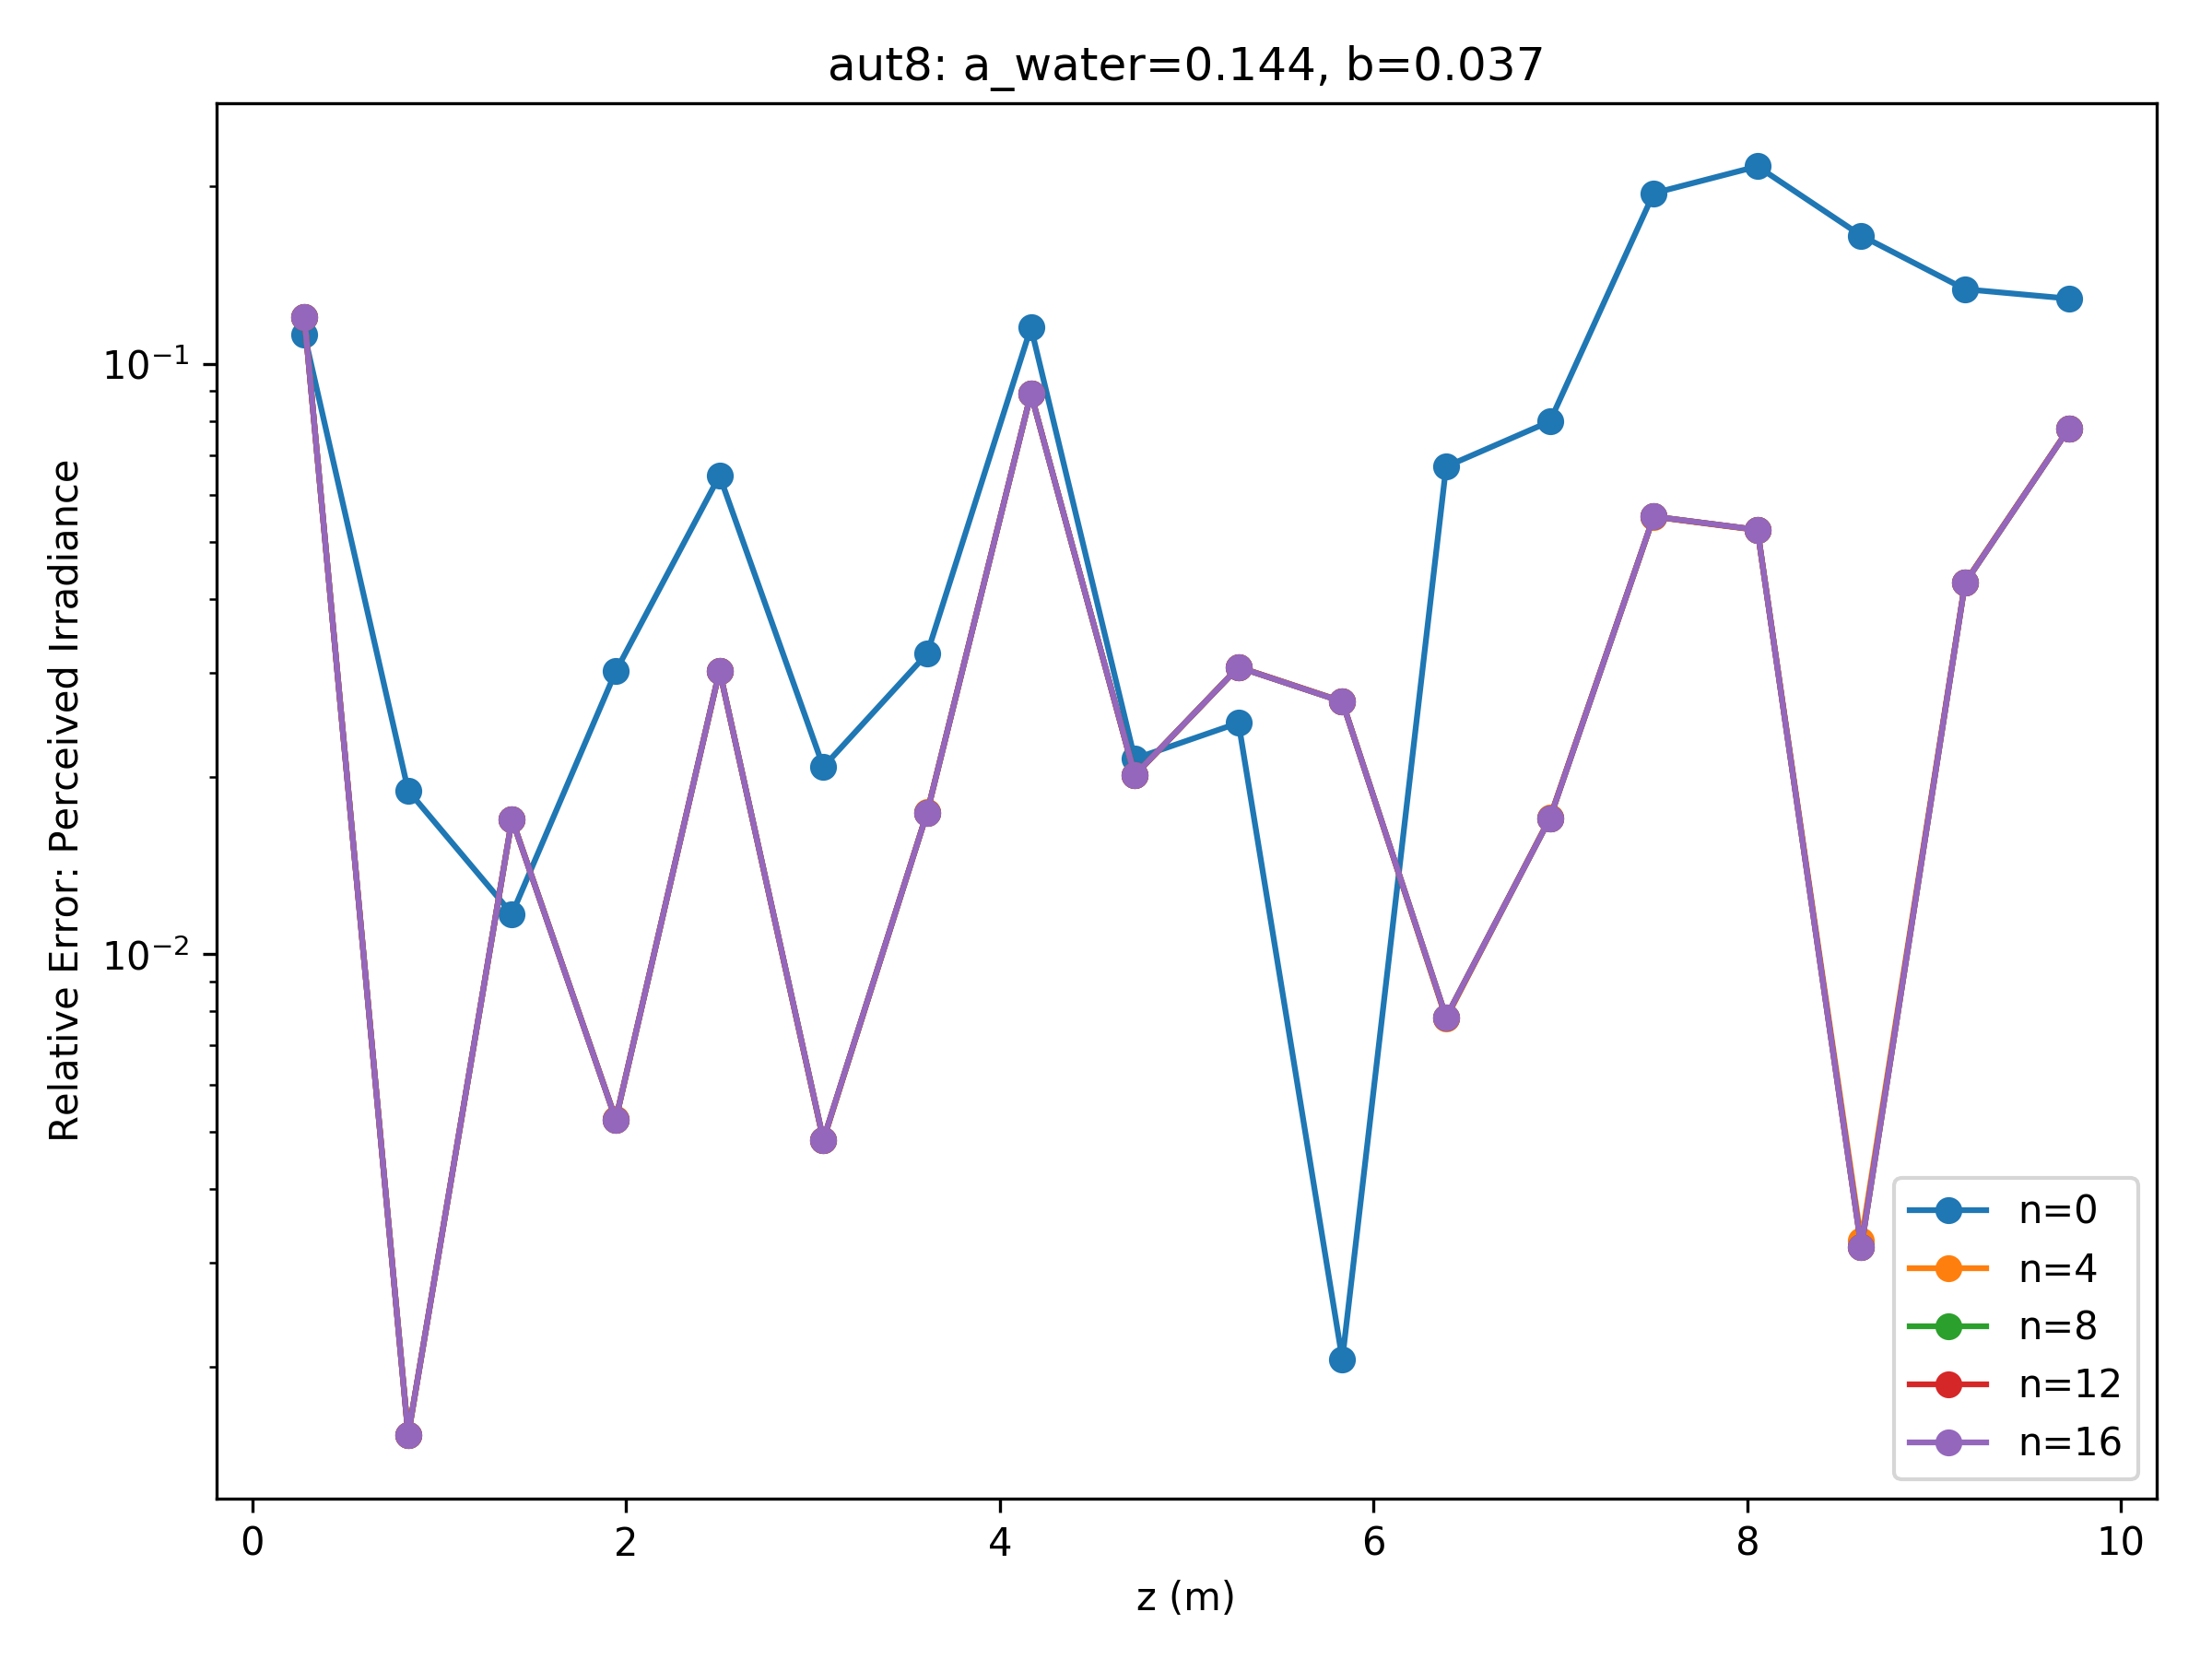
\includegraphics[width=4in]{asym_conv_rel_err_aut8}
  \caption{Successive asymptotic approximations, relative error: AUT8}
\end{figure}

%%

\begin{figure}[H]
  \centering
  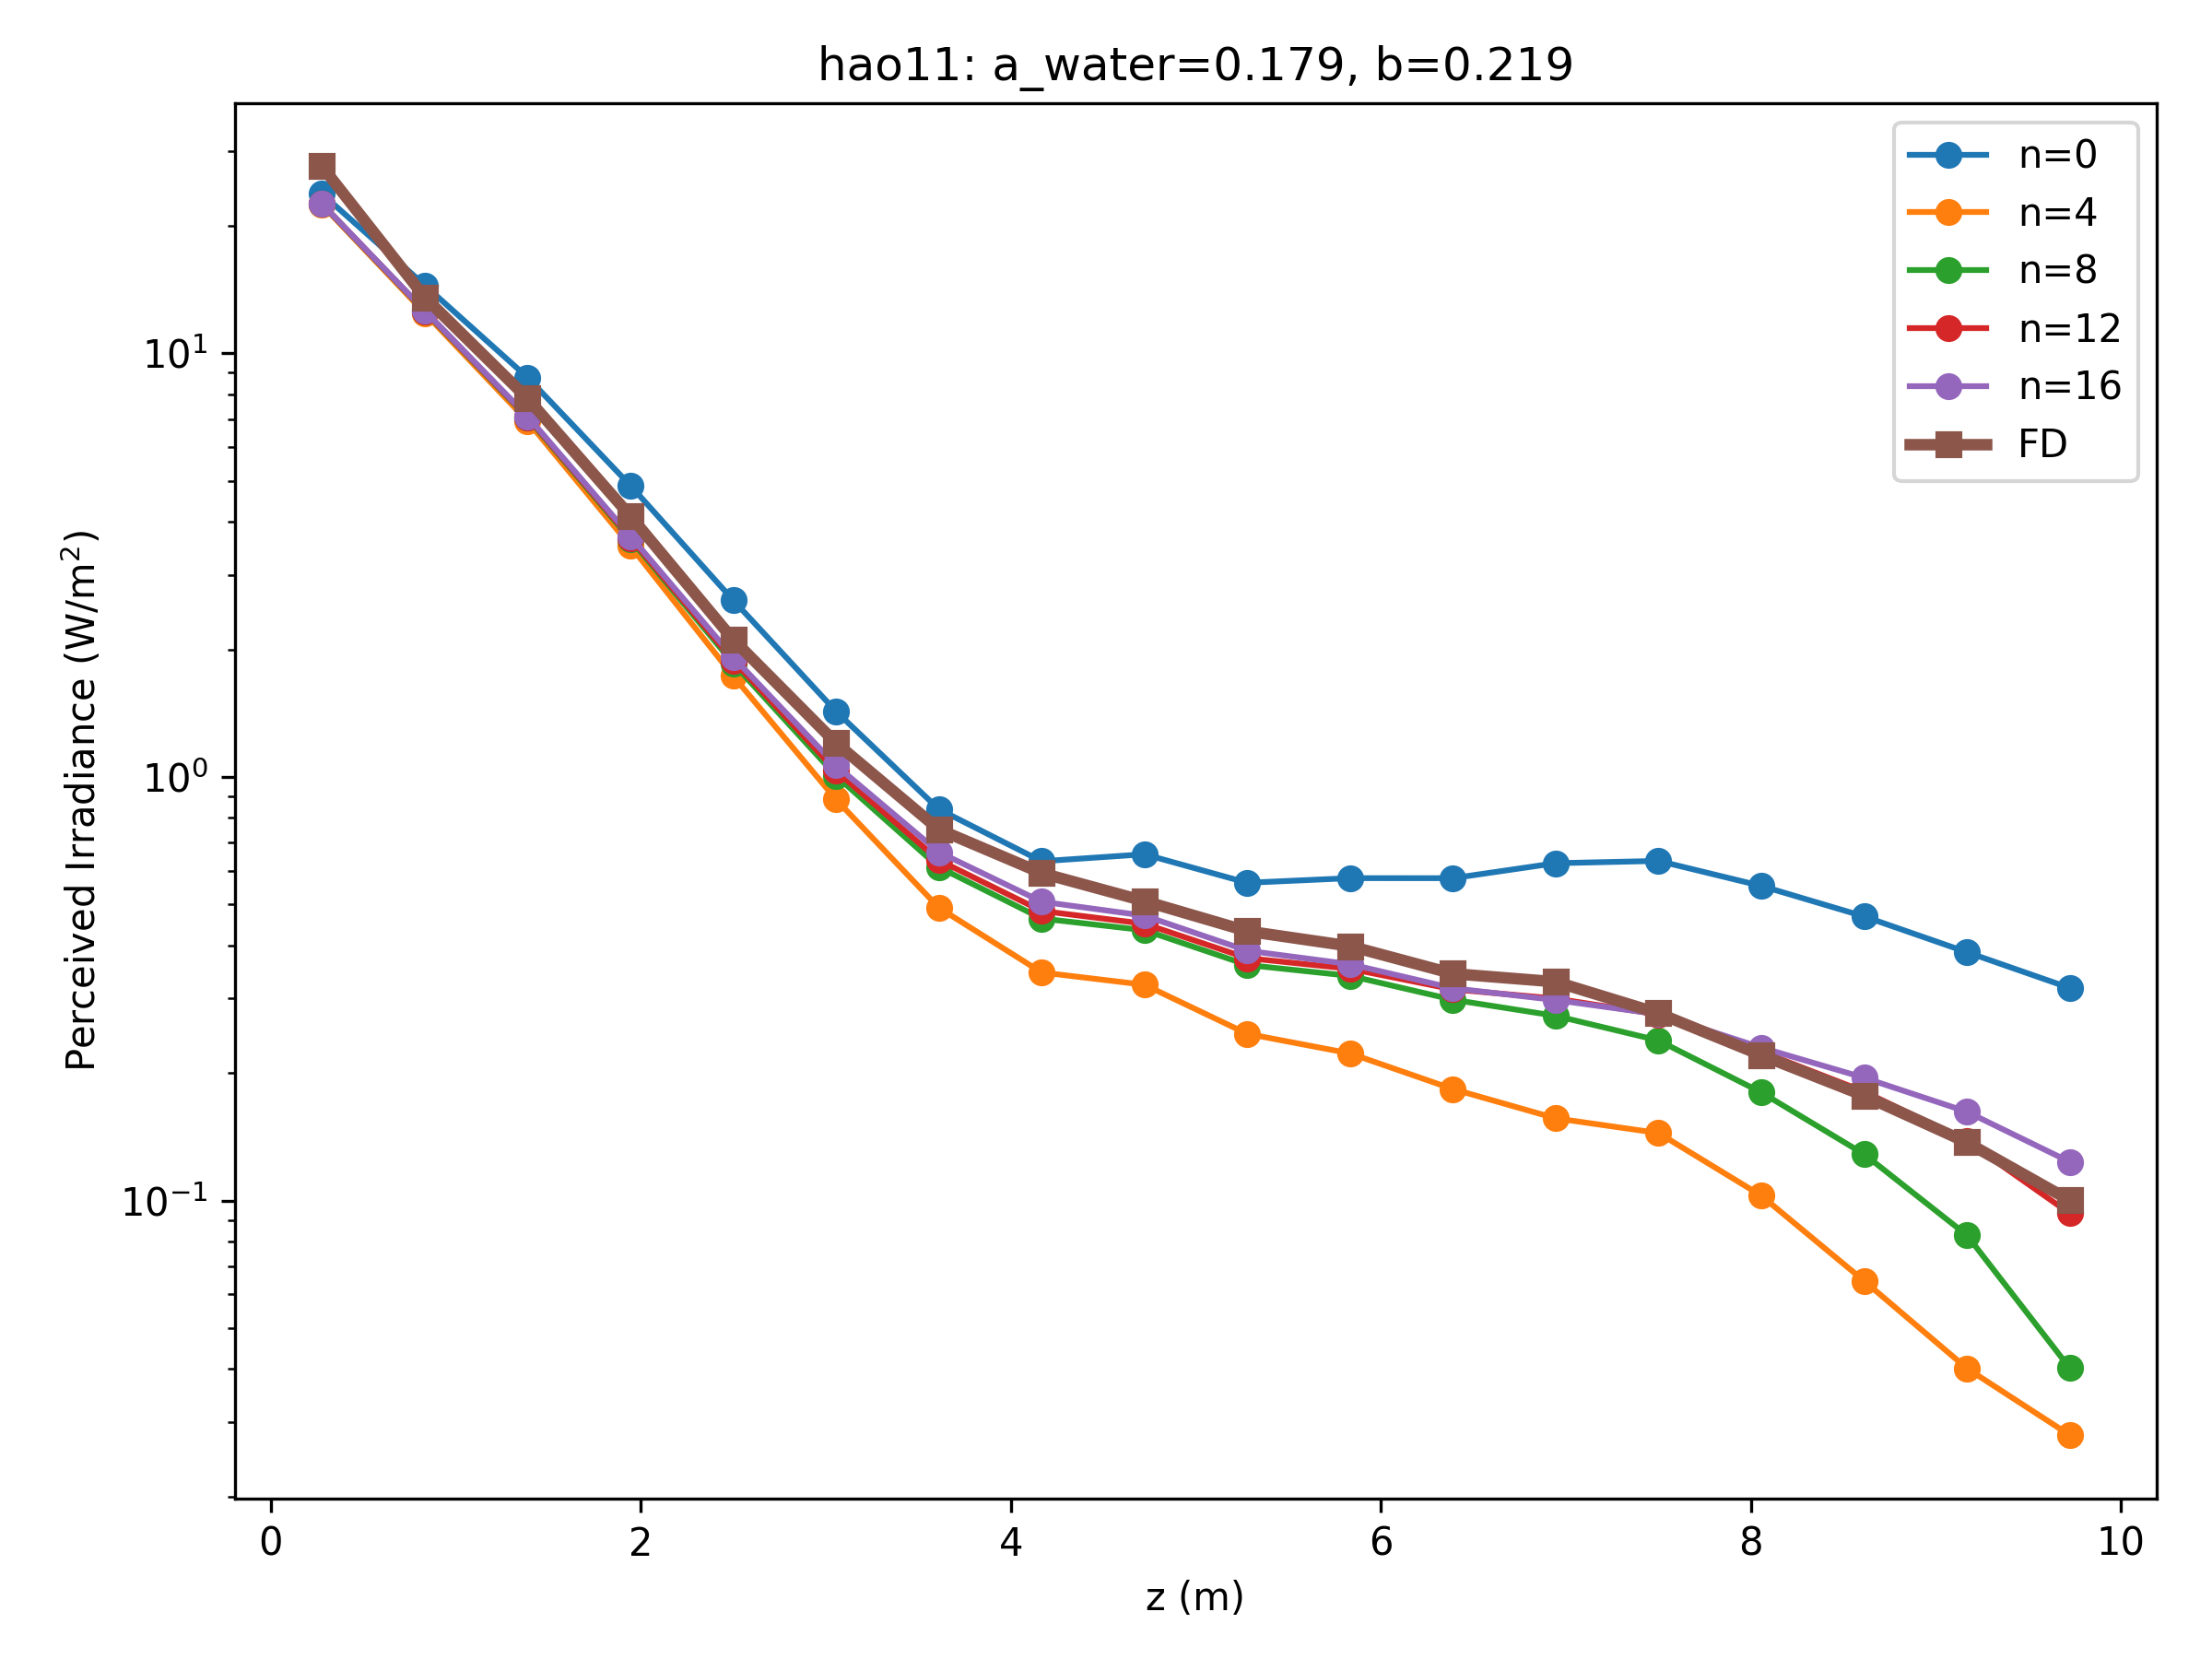
\includegraphics[width=4in]{asym_conv_irrad_hao11}
  \caption{Successive asymptotic approximations, irradiance: HAO11}
\end{figure}

\begin{figure}[H]
  \centering
  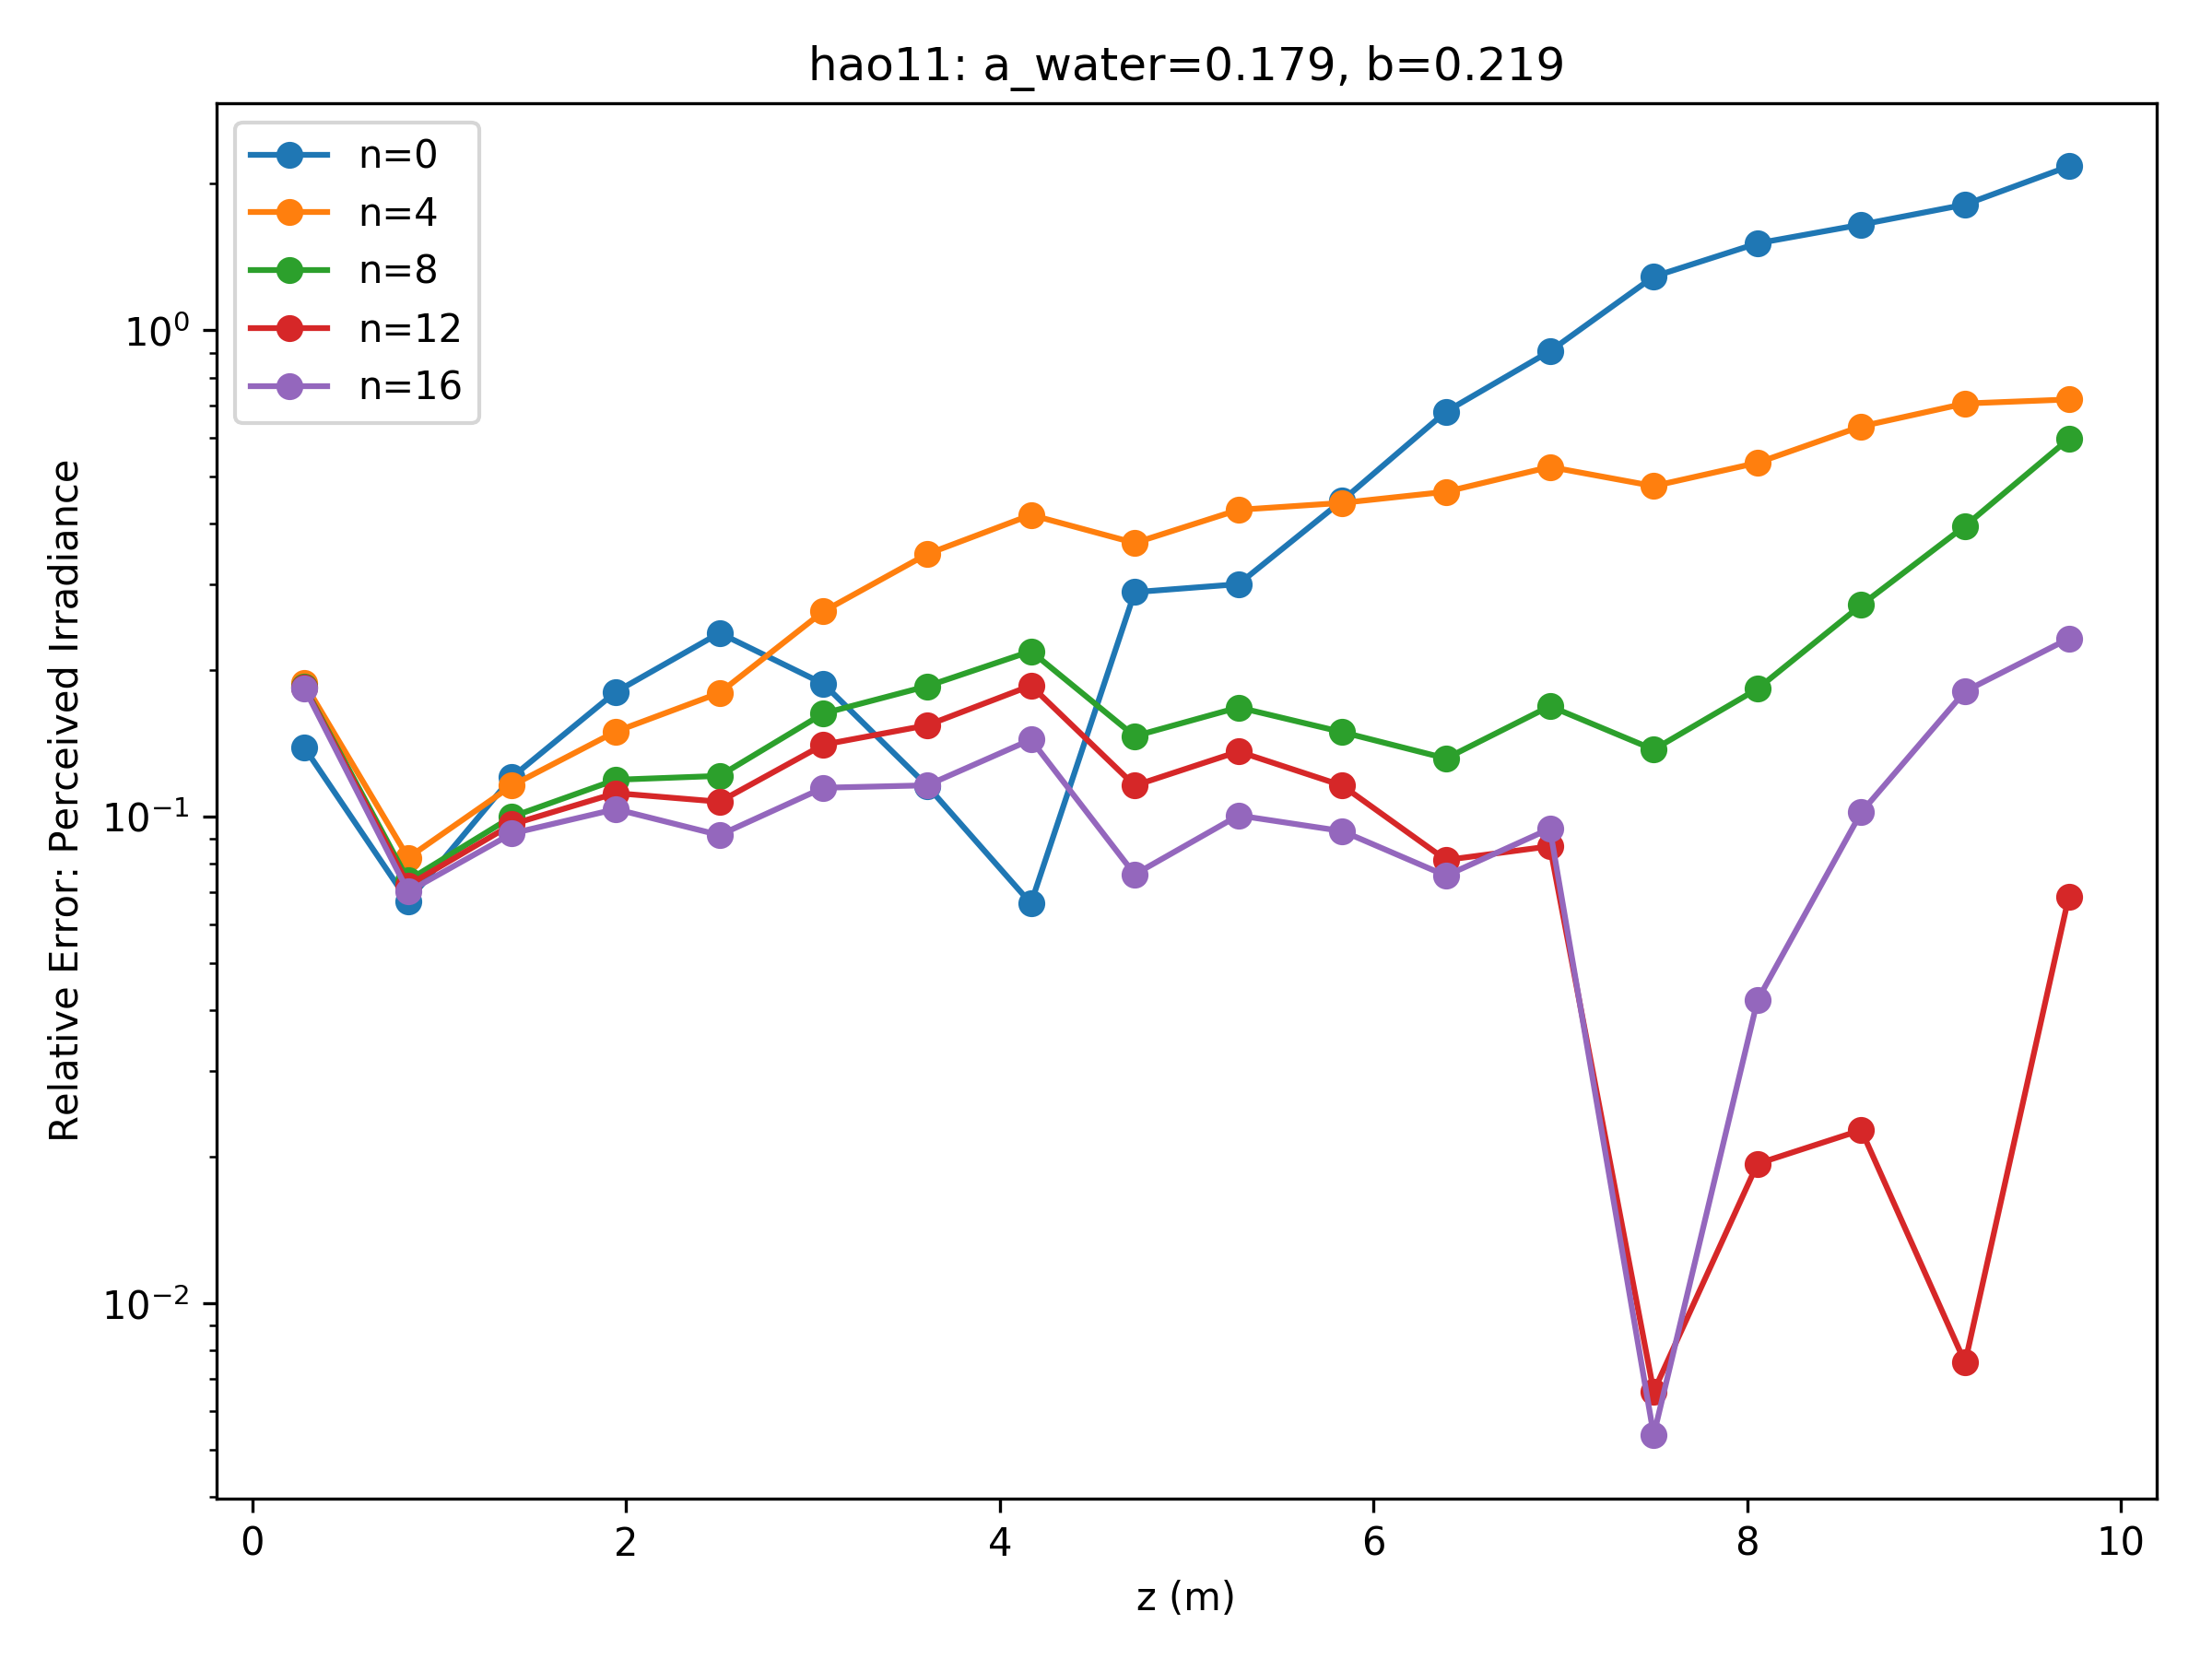
\includegraphics[width=4in]{asym_conv_rel_err_hao11}
  \caption{Successive asymptotic approximations, relative error: HAO11}
\end{figure}

%%

\begin{figure}[H]
  \centering
  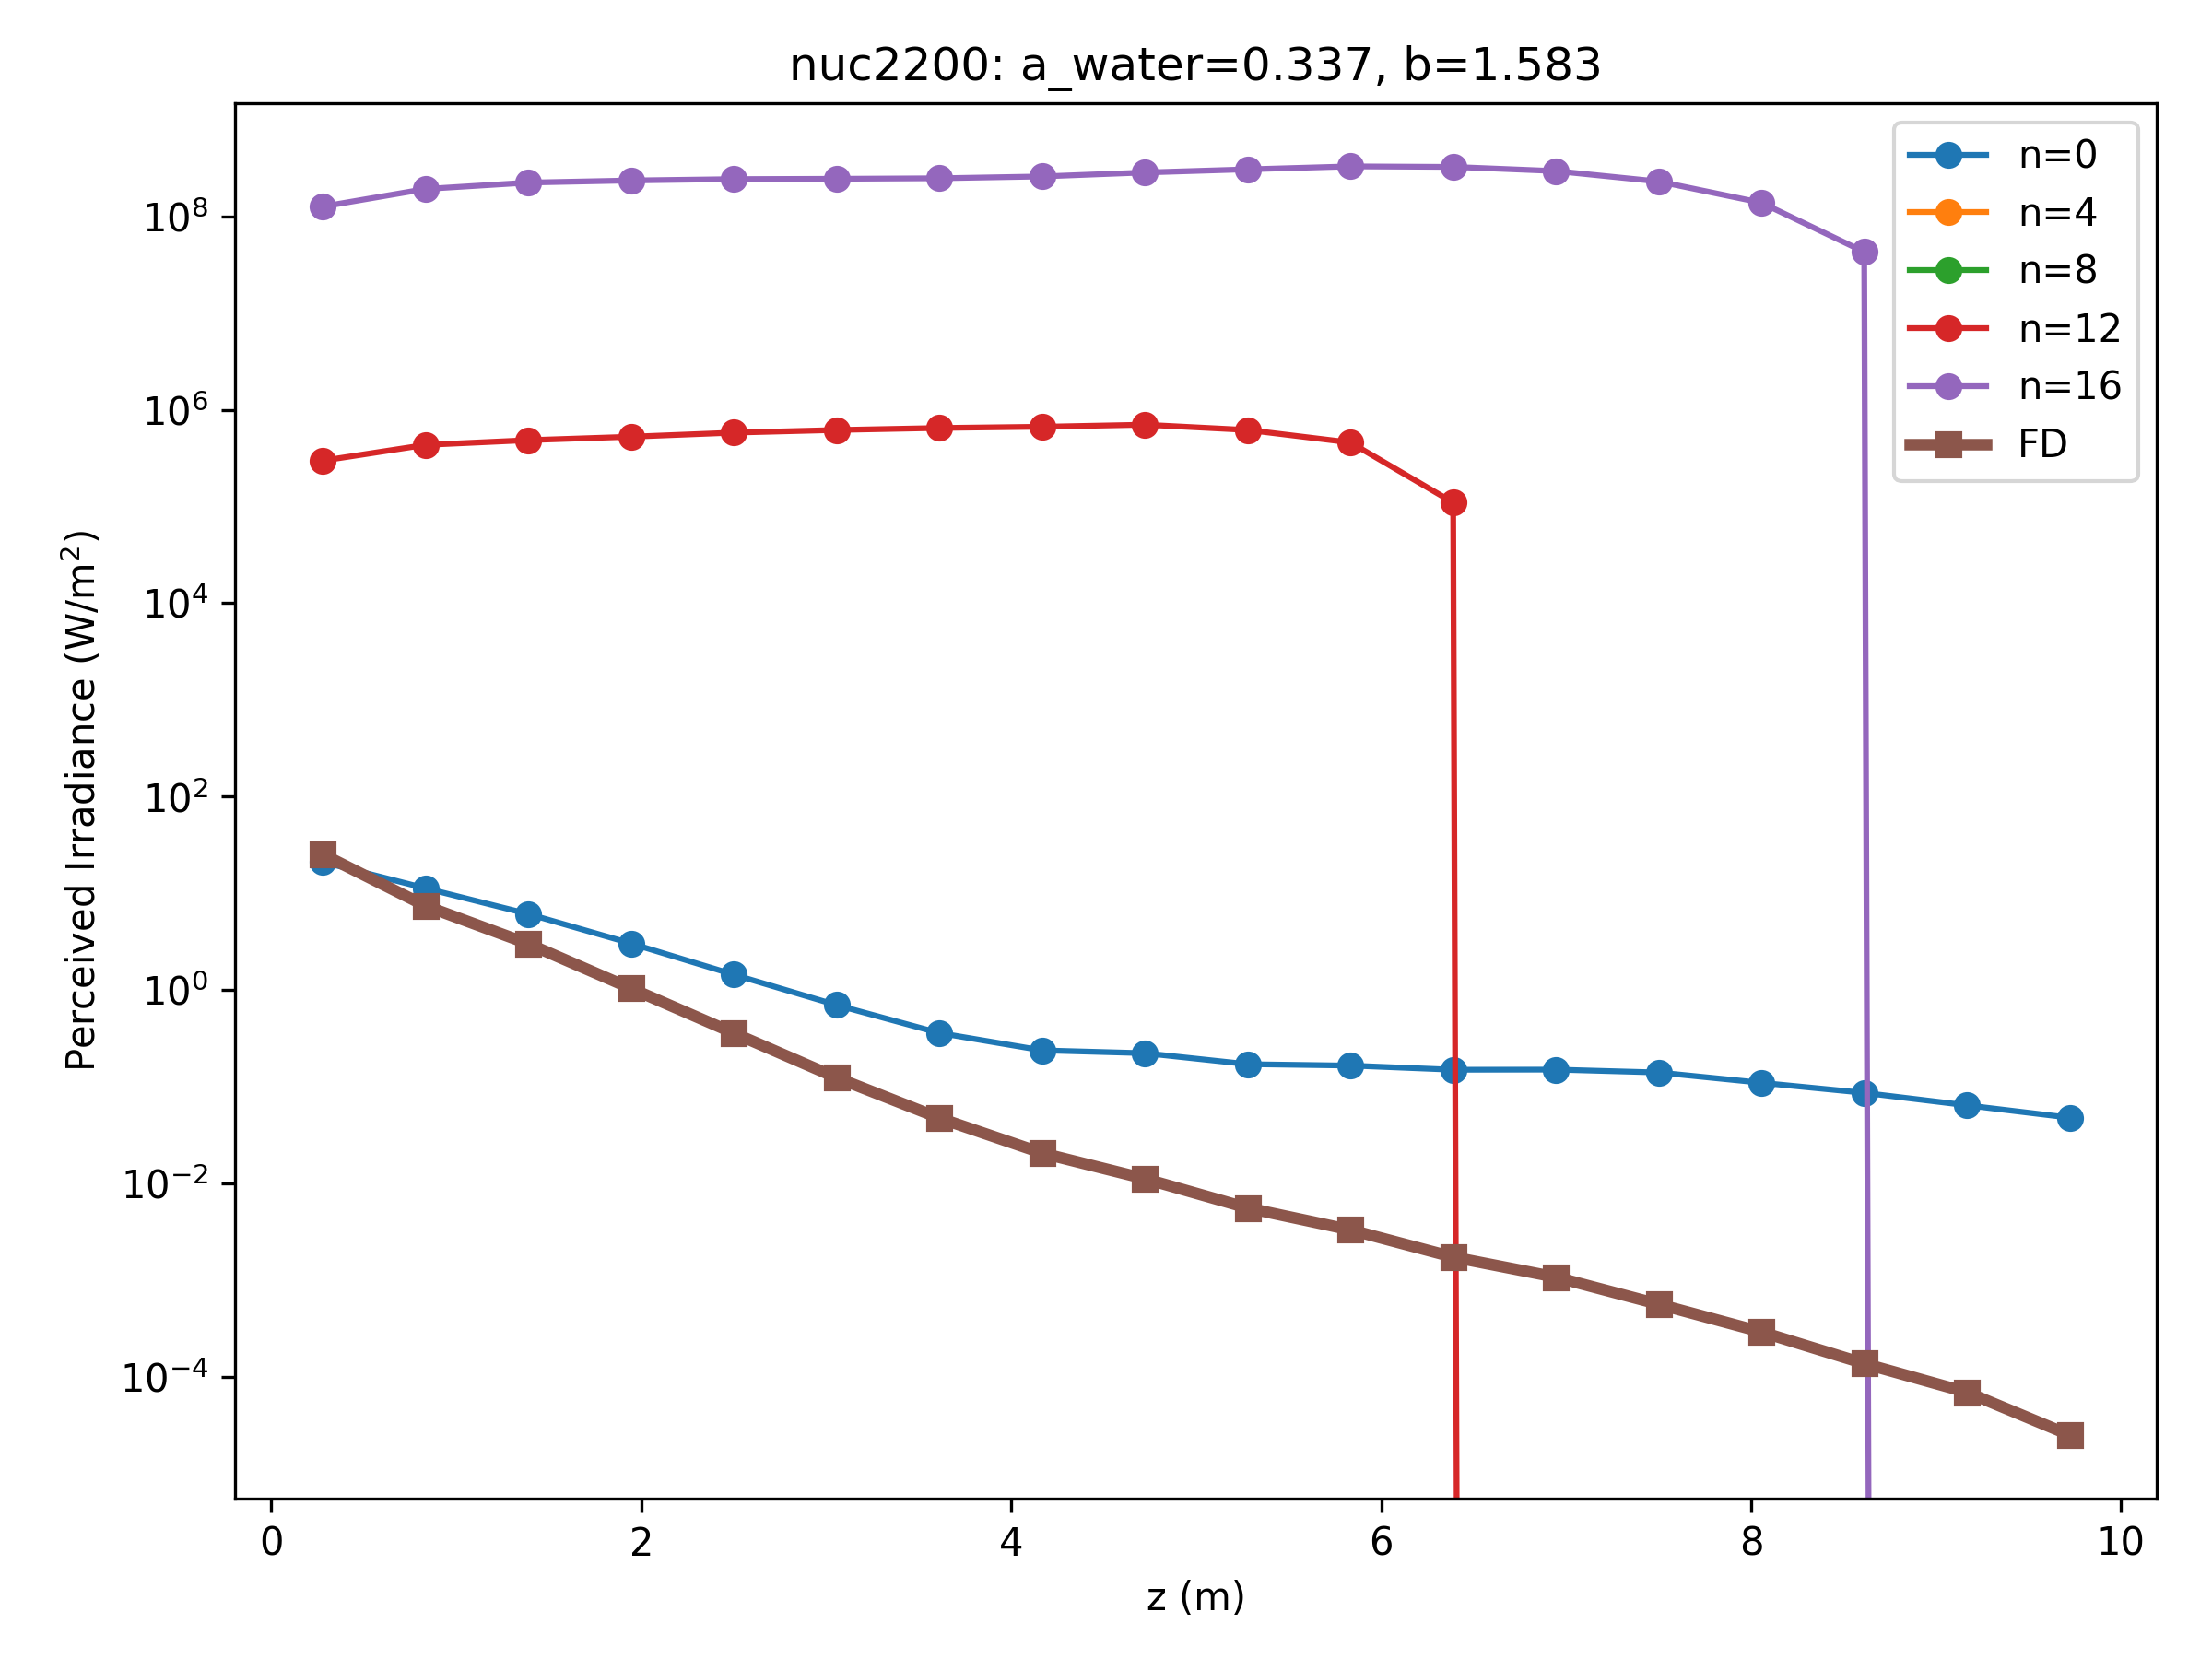
\includegraphics[width=4in]{asym_conv_irrad_nuc2200}
  \caption{Successive asymptotic approximations, irradiance: NUC2200}
\end{figure}

\begin{figure}[H]
  \centering
  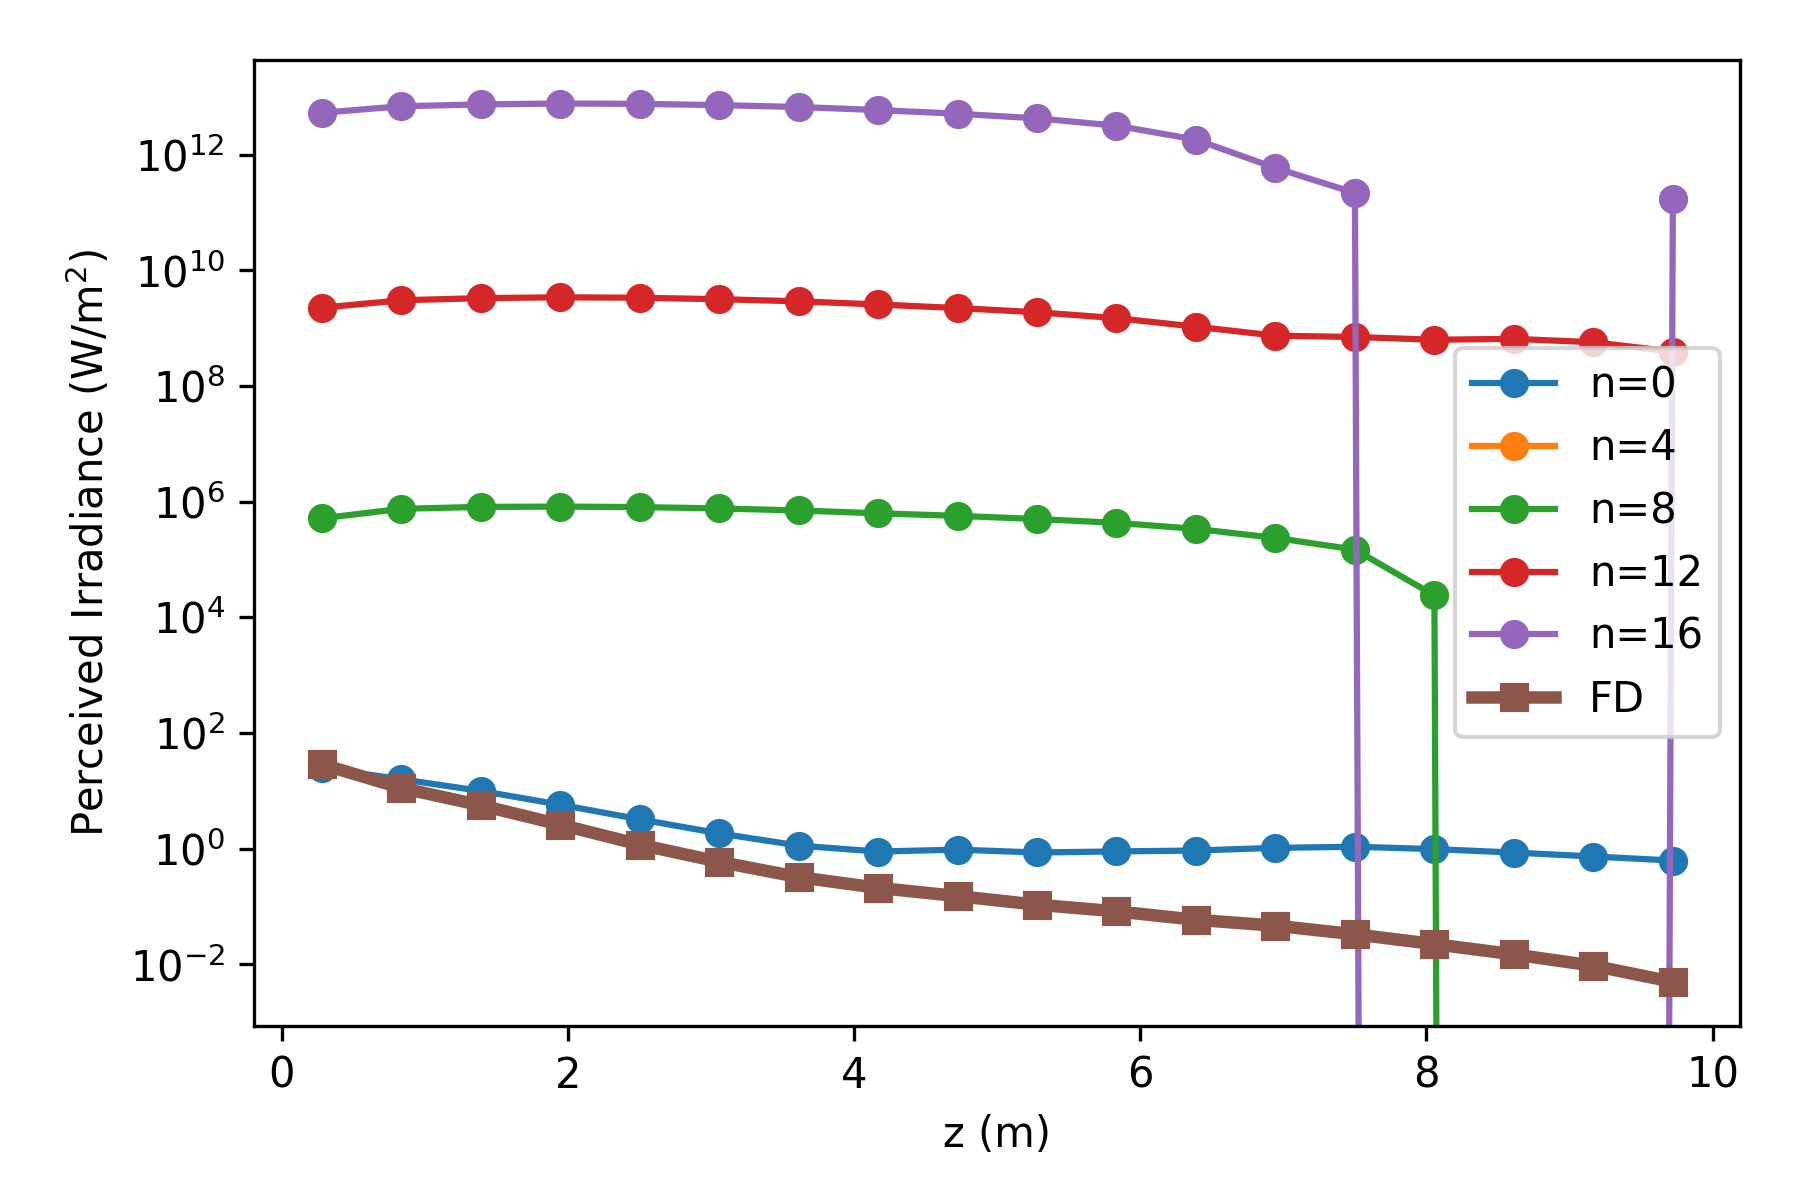
\includegraphics[width=4in]{asym_conv_irrad_nuc2240}
  \caption{Successive asymptotic approximations, relative error: NUC2240}
\end{figure}

%%

\begin{figure}[H]
  \centering
  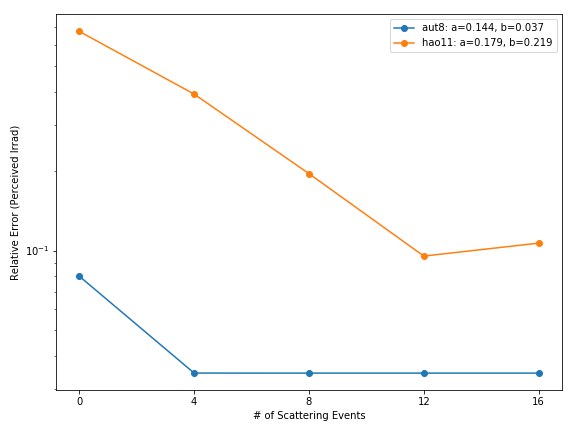
\includegraphics[width=4in]{asym_conv_compare}
  \caption{Comparison of asymptotic approximations for various waters.}
  \label{fig:asym_conv_compare}
\end{figure}

\section{Sensitivity Analysis}
In this section, we demonstrate the effect of varying some of the parameters of the model.
The 12-term asymptotic approximation is used.
In Figure \ref{fig:sens_analysis_a_water} and Figure \ref{fig:sens_analysis_b}, the solution
is shown to diverge when the ratio $b/a$ is too large, as in Section \ref{sec:asym_conv}.

\begin{figure}[H]
  \centering
  \vspace{-3em}
  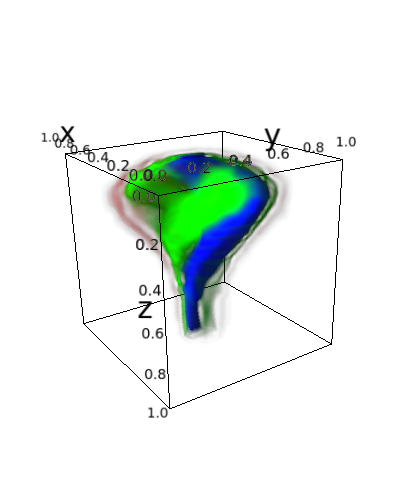
\includegraphics[width=0.45\textwidth]{top-heavy_kelp}
  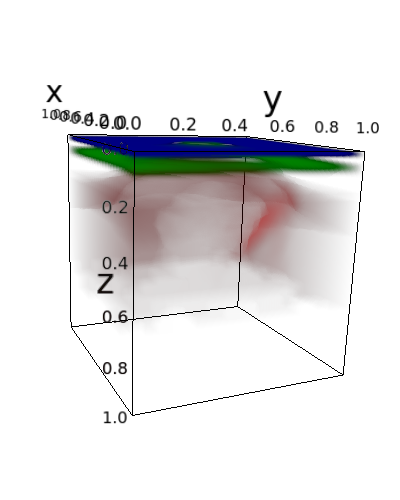
\includegraphics[width=0.45\textwidth]{top-heavy_irrad}
  \caption{\textit{top-heavy} kelp distribution (left) and no-scattering irradiance profile (right)}
\end{figure}

\begin{figure}[H]
  \centering
  \vspace{-3em}
  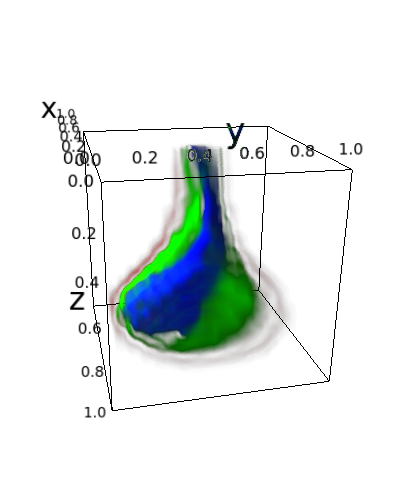
\includegraphics[width=0.45\textwidth]{bottom-heavy_kelp}
  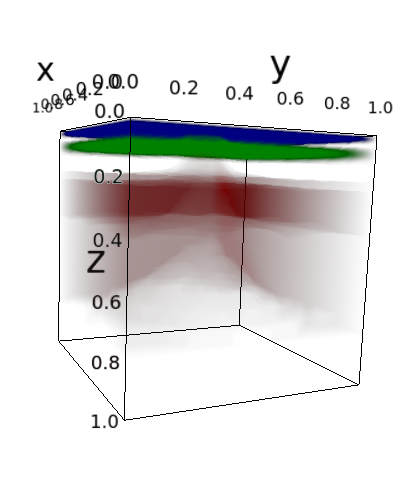
\includegraphics[width=0.45\textwidth]{bottom-heavy_irrad}
  \caption{\textit{bottom-heavy} kelp distribution (left) and no-scattering irradiance profile (right)}
\end{figure}

\begin{figure}[H]
  \centering
  \vspace{-3em}
  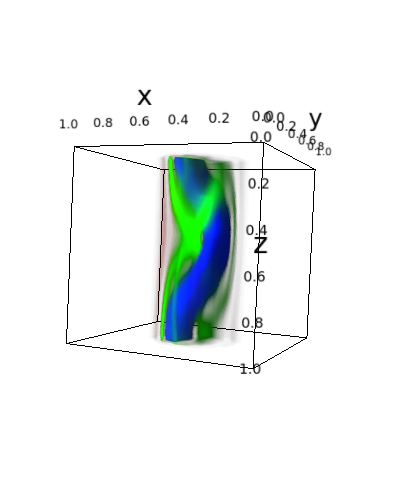
\includegraphics[width=0.45\textwidth]{uniform_kelp}
  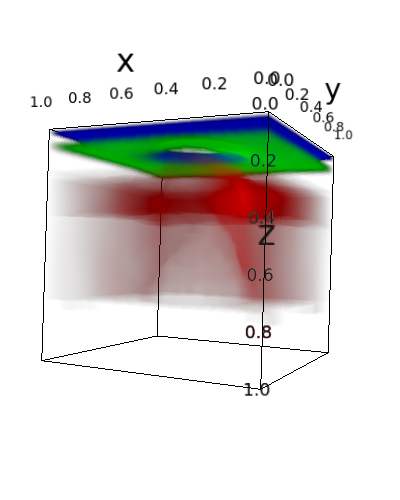
\includegraphics[width=0.45\textwidth]{uniform_irrad}
  \caption{\textit{uniform} kelp distribution (left) and no-scattering irradiance profile (right)}
\end{figure}

\begin{figure}[H]
  \centering
  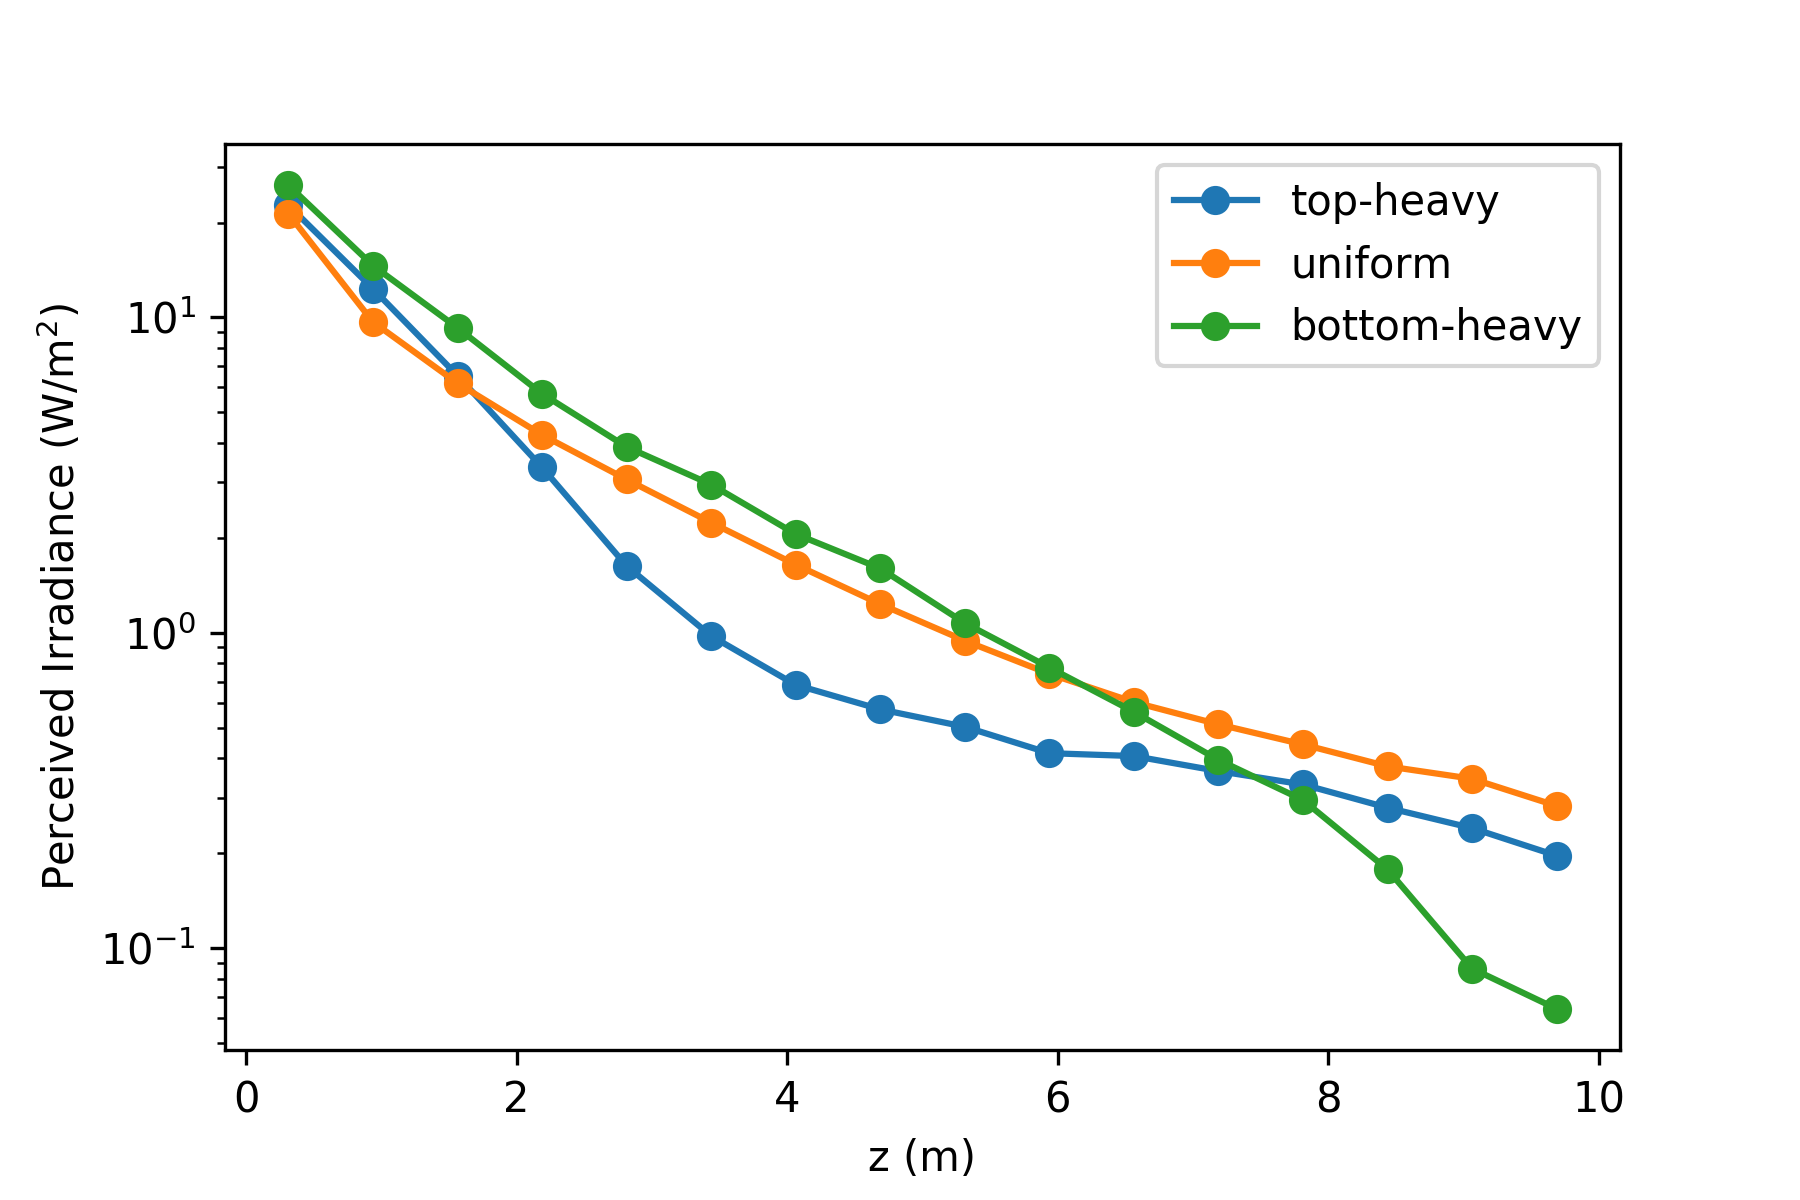
\includegraphics[width=4in]{sens_analysis_kelp_profile}
  \caption{Several kelp profiles}
\end{figure}

\begin{figure}[H]
  \centering
  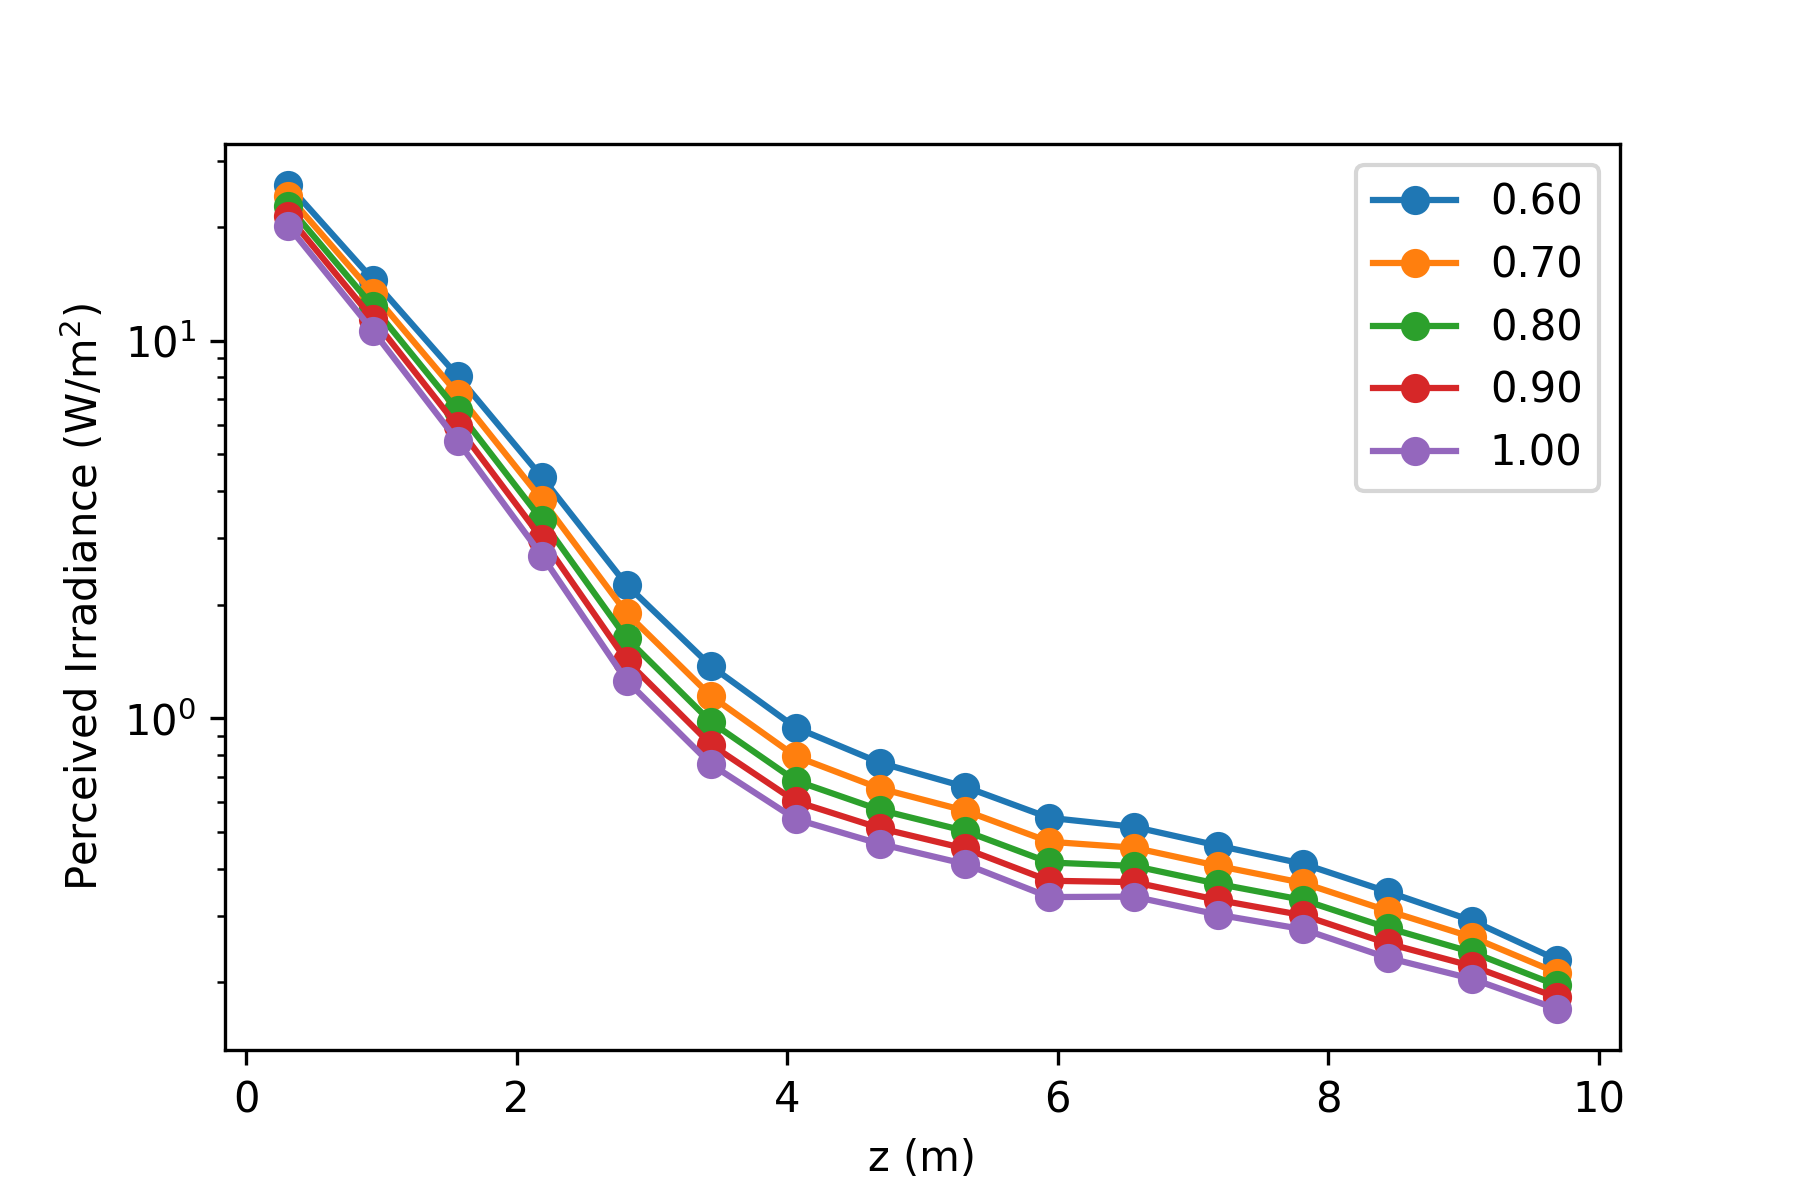
\includegraphics[width=4in]{sens_analysis_absorptance_kelp}
  \caption{Several values of kelp absorptance}
\end{figure}

\begin{figure}[H]
  \centering
  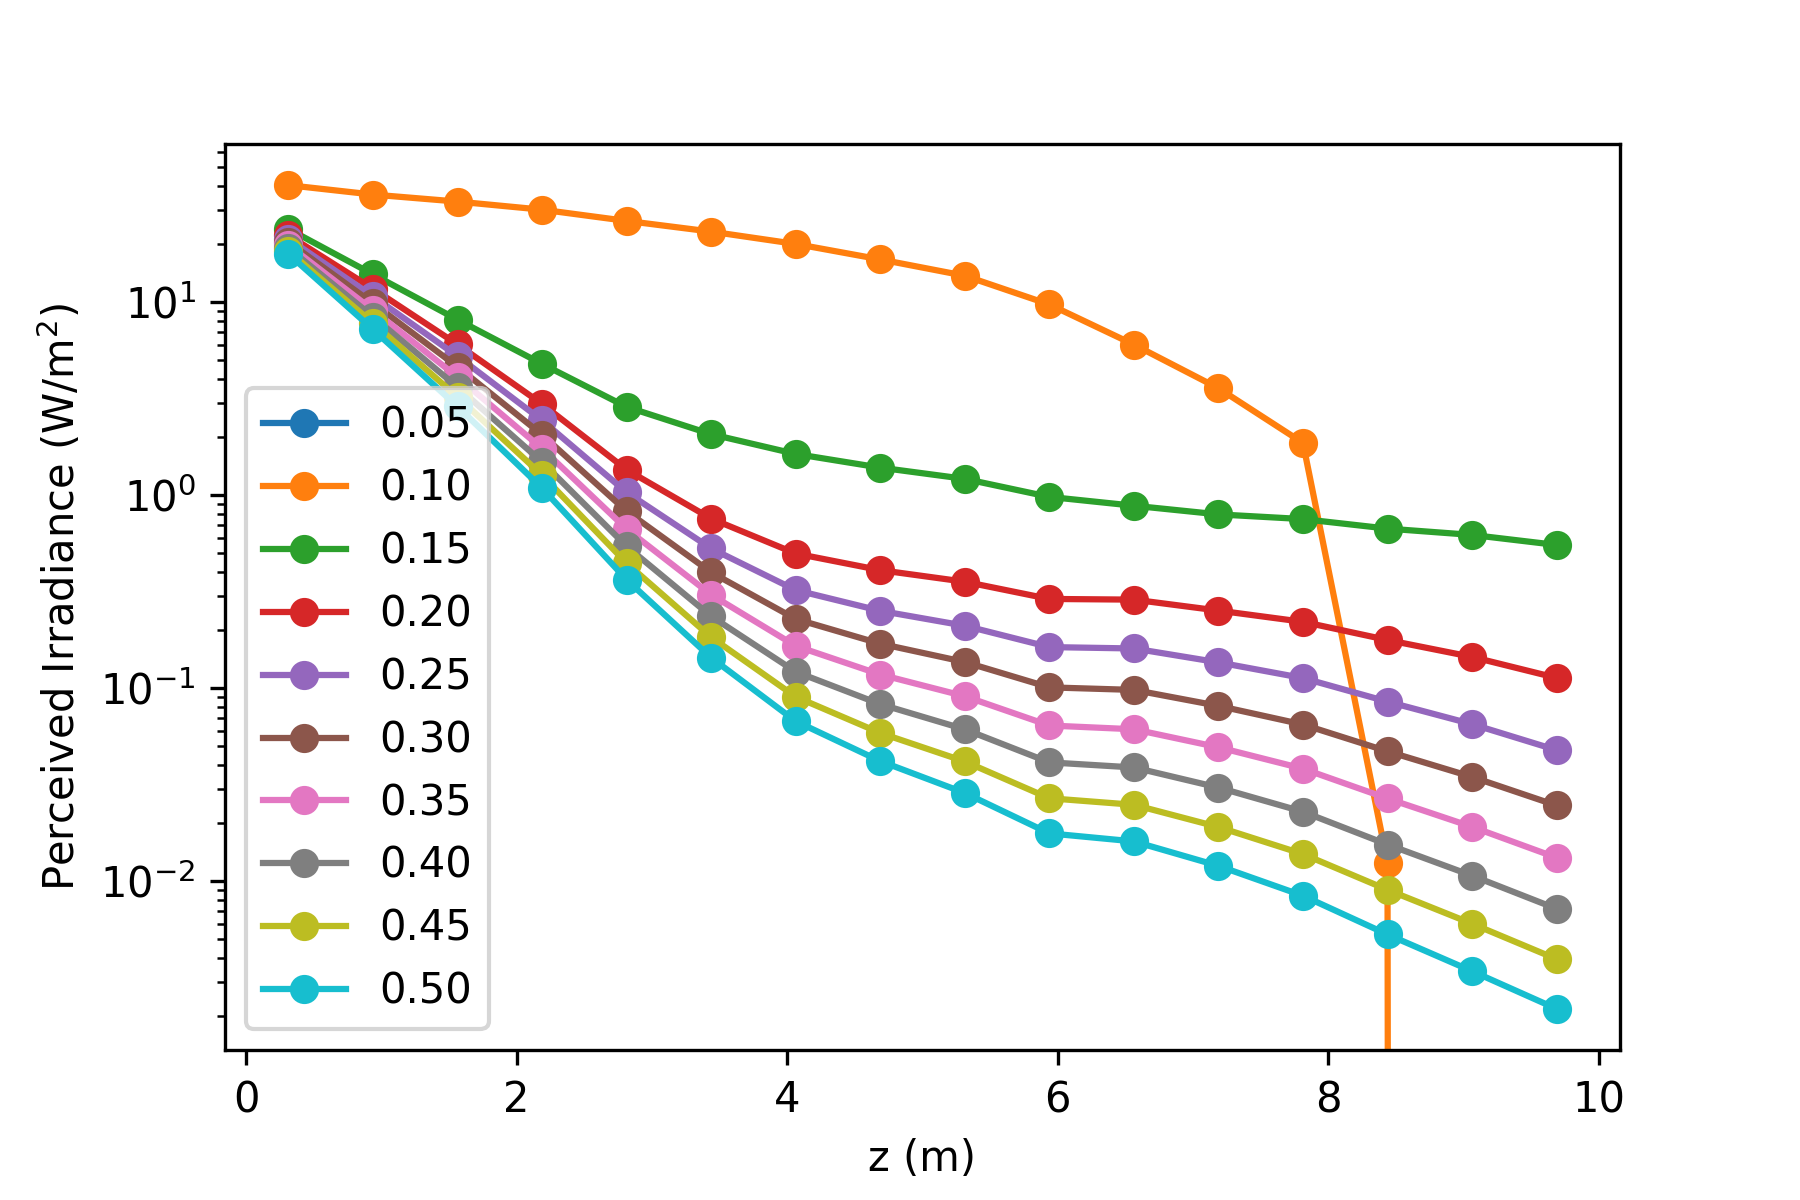
\includegraphics[width=4in]{sens_analysis_a_water}
  \caption{Several values of absorption coefficient of water}
  \label{fig:sens_analysis_a_water}
\end{figure}

\begin{figure}[H]
  \centering
  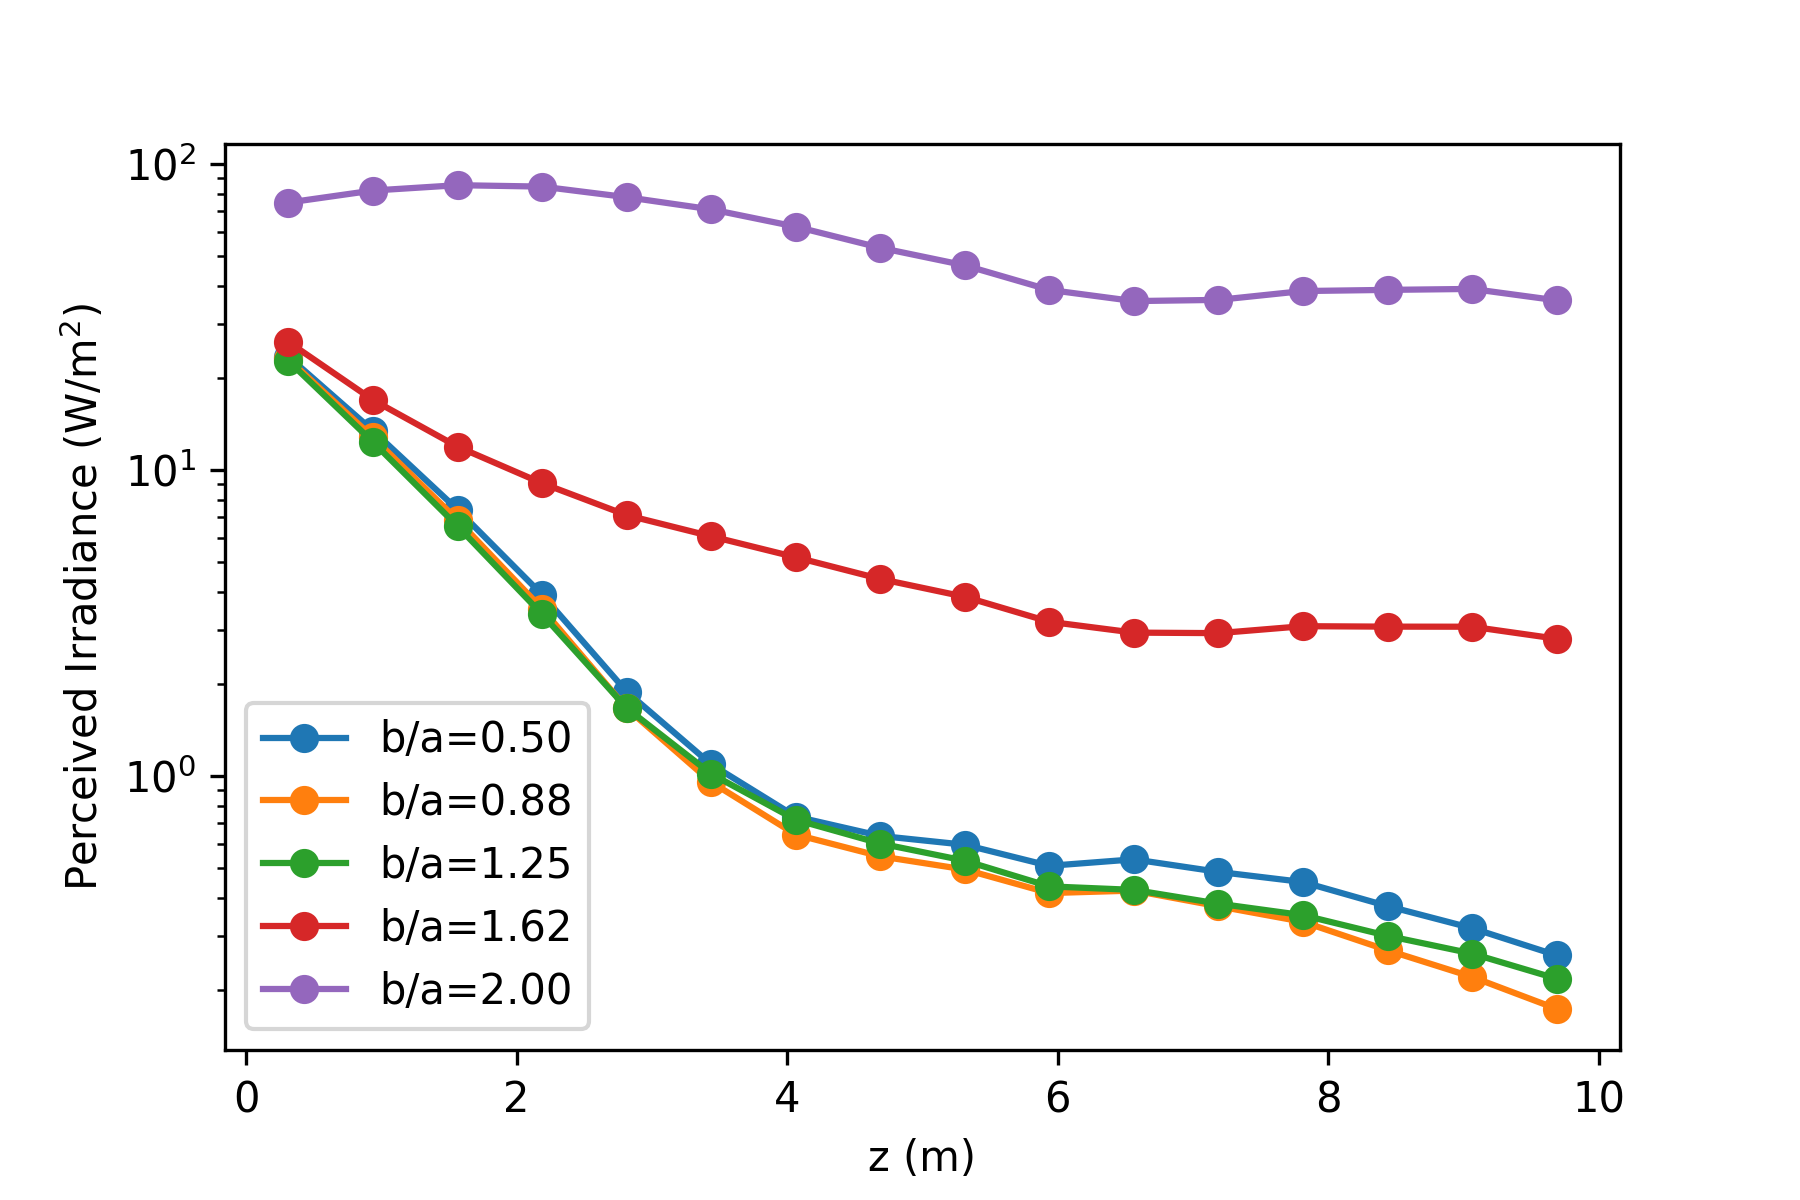
\includegraphics[width=4in]{sens_analysis_b}
  \caption{Several values of scattering coefficient}
  \label{fig:sens_analysis_b}
\end{figure}
